% Preamble of a dissertation
% Preamble of a dissertation
\documentclass[a4paper,twoside, openany]{book}
\pagestyle{empty}
  \linespread{1.5}
\usepackage[left=2cm,right=2cm,top=3cm,bottom=2cm]{geometry}
\usepackage[portuguese,main=english]{babel}
\usepackage[latin1,utf8]{inputenc}
\usepackage{hyperref}
\hypersetup{
    colorlinks=true,
    linkcolor={black},      % color of internal links
    citecolor=[rgb]{0.03,0.27,0.49},      % color of links to bibliography
    filecolor=[rgb]{0.00,0.50,0.00},      % color of file links
    urlcolor=[rgb]{0.10,0.30,0.90},       % color of external links
}
\usepackage[T1]{fontenc}
\usepackage{amsmath,amsfonts,amssymb,latexsym,amstext,amsbsy,amsthm}
\usepackage{mathtools}
\usepackage{pdflscape}
\usepackage{rotating}
\usepackage{everypage}
\usepackage[toc,page]{appendix}
\usepackage{graphicx}
\usepackage[space]{grffile}
\usepackage[round]{natbib}
\usepackage{array} % for tables with fixed length
\usepackage{tocloft}
\usepackage{booktabs}
\usepackage[table,xcdraw]{xcolor}
\usepackage{longtable}
\usepackage{tablefootnote}
\usepackage{threeparttablex}
\usepackage{filecontents}
\usepackage{pdfpages}
%\parindent 3ex
\usepackage[footnotesize,labelsep=space,sl]{caption}
\usepackage{setspace}
\usepackage{url}
\usepackage{fancyhdr}% http://ctan.org/pkg/fancyhdr
\fancypagestyle{frontmatter}{%
  \renewcommand{\headrulewidth}{0pt}% No header rule
  \renewcommand{\footrulewidth}{0pt}% No footer rule
  \fancyhf{}% Clear header/footer
  \fancyfoot[C]{\thepage}%
}
\fancypagestyle{mainmatter}{%
  \renewcommand{\headrulewidth}{.4pt}% Header rule
  \renewcommand{\footrulewidth}{.4pt}% Footer rule
  \fancyhf{}% Clear header/footer
  \fancyhead[L]{\leftmark}% Chapter in header Left
  \fancyhead[R]{\thepage}% Page number in header Right
}
\usepackage{epigraph}

\newcommand{\ok}{$\checkmark$}



\begin{document}
	% Cover page, Title, Dedication, Acknowledgements, Abstract, Resumo
	% Contents, List of Tables, List of Figures
\frontmatter
\pagestyle{frontmatter}% frontmatter page style
\begin{spacing}{1.5}
	
	%Cover page and Title
	\pagenumbering{roman}
		\begin{titlepage}
		\begin{center}
			\vspace*{0.5cm}
			\Large{Universidade de S\~{a}o Paulo}\\
			\Large{Instituto de Astronomia, Geof\'{i}sica e Ci\^{e}ncias Atmosf\'{e}ricas}\\
			\Large{Pos-Gradua\c{c}\~{a}o em Meteorologia}\\[3cm]
			Alejandro Herman Delgado Peralta \\[3cm]

			\huge{\textbf{Simulation of Tropospheric Ozone Formation in the Metropolitan Area of S\~{a}o Paulo under Climate Change Scenarios}}\\[3mm]
			\vfill

			S\~{a}o Paulo \\
			\the\year \\
			
		\end{center}
	\end{titlepage}
	
	\newpage
	\thispagestyle{empty}
		% Face page
	\begin{titlepage}
		\begin{center}
			\vspace*{0.5cm}
			\Large{Alejandro Herman Delgado Peralta}\\[4cm]

			\huge{\textbf{Simulation of Tropospheric Ozone Formation in the Metropolitan Area of S\~{a}o Paulo under Climate Change Scenarios}}\\[4cm]
		\end{center}
		\hfill\begin{minipage}{0.5\linewidth}
		Dissertation submitted to "Instituto de Astronomia, Geof\'{i}sica e Ci\^{e}ncias Atmosf\'{e}ricas" (IAG) of the "Universidade de S\~{a}o Paulo". It is a partial requirement to obtain a Master's degree in Science.\\[1cm]
				Concentration area: Meteorology\\
				Advisor: Prof.$^a$ Dr.$^a$ Maria de F\'{a}tima Andrade
		\end{minipage}
	
			\vfill
	\begin{center}
				S\~{a}o Paulo \\
			\the\year \\
	\end{center}
	\end{titlepage}		

	% Dedication
	\newpage
	\thispagestyle{empty}
	\vspace*{\fill} \hfill\begin{minipage}{0.5\linewidth}
	\begin{flushright}
	\textit{This dissertation work is dedicated to my parents for their love and those who have committed to science.  \\
	\#NoScienceNoFuture\\
	\#SinCienciaNoHayFuturo \\
	 }
	\end{flushright}
		\end{minipage}
	\pagestyle{empty}
	
	% Acknowledgements
	\newpage
	\phantomsection\addcontentsline{toc}{chapter}{Acknowledgements}
		\begin{center}
			\LARGE \textbf{Acknowledgements}\\[2cm]
		\end{center}
		
		This research was made possible by the CAPES (\textit{Coordena\c{c}\~{a}o de Aperfei\c{c}onamento de Pessoal de N\'{i}vel Superior}), who funded the work during the master's studies.
		The University of S\~{a}o Paulo through the Institute of Astronomy, Geophysics and Atmospheric Sciences, and the laboratory LAPAt, supported this work by providing its facilities as a computer server and the remote connection during the pandemic.
		I also thank the State Company for the Environment (CETESB) for providing free hourly data from its station network available on its website (QUALAR).
		I am very grateful to the following people for supporting and encouraging me; without whose help, this work would never have been possible:
		\begin{itemize}
		    \item Prof.($^a$) Dr.($^a$) Maria de F\'{a}tima Andrade, who gave me many valuable insights in all stages of this work.
		    Professors responsible of each master's courses and during the qualification exam: Adalgiza Fornaro, Edmilson Dias de Freitas, Maria Assun\c{c}\~{a}o Faus da Silva Dias, M\'{a}rcia Akemi Yamasoe, Ricardo Hallak, and Rita Yuri Ynoue.
		   \item  My friends Dr. Angel Vara Vela and Dr. Mario Gavidia Calder\'{o}n for their valuable suggestions, discussions, support, and teaching related to the WRF-Chem model (setup, create emission files, and post-processing).
		   \item To my friends Angela Ascarza and Guisselle Castillo for the proofreading of the English writing.
		   \item I also acknowledge Dr. Pieter Tans (NOAA/GML) and Dr. Ralph Keeling (Scripps Institution of Oceanography) for the permission to use the CO$_2$ trend plots.
		\end{itemize}
		
		Also, I would like to thank my family (especially my wife and my little cat) for their support and encouragement to successfully address this challenge.
		Finally, thanks to those friendly people to make my life more comfortable during my stay in Brazil and at the University of S\~{a}o Paulo.
		
		\textbf{Thank God for good memories,		
		\textit{muito obrigado},
      	\textit{muchas gracias}}.
		
		
		\cleardoublepage
	
	% Abstract
	\phantomsection\addcontentsline{toc}{chapter}{Abstract}
	\begin{center}
		\LARGE \textbf{Abstract}\\[2cm]
	\end{center}
	% main objective: impact of future climate change scenarios on o3 in the MASP
    % Specific objectives: Prepare and updated emissions file and model configuration
    % Specific objectives: Evaluation of WRF-Chem and simultations based on RCP scenarios. study current conditions that affect the tropospheric ozone formation through the WRF-Chem model compared with observations. Study how changes in future meteorological conditions impact the surface ozone formation in the MASP and around it.
    %%%%%%%%%%%%%%%%%%%%%%%%%%%%%%%%%%%%
The impact on ozone formation in the Metropolitan Area of S\~{a}o Paulo (MASP) in 2030 was analyzed through two atmospheric projections based on the Representative Concentration Pathway (RCP) emission scenarios. The modeling system applied in this study was the Weather Research and Forecasting with Chemistry (WRF-Chem) model, maintaining the same emission rates in the MASP and surroundings from road transport, industry, and residential sectors of the base year of 2018.
The study of tropospheric ozone (O$_3$) has a particular interest in air quality and climate change due to its importance as an atmospheric pollutant and a greenhouse gas.
It was considered three simulations, corresponding to a control period (Sep-Oct 2018), and two projected scenarios for Sep.-Oct. 2030 based on the RCP emission projections for 4.5 and 8.5 W~m$^{-2}$ as radiative forcing.
We evaluated the model performance for surface ozone and meteorological parameters using available hourly measurements from the \textit{Companhia de Tecnologia de Saneamento Ambiental} (CETESB, Environmental Protection Agency) and the \textit{Instituto de Astronomia, Geof\'{i}sica e Ci\^{e}ncias Atmosf\'{e}ricas} (IAG) Climatological Station. Also, emissions representativeness for September and October 2018 were verified through the WRF-Chem model using a configuration based on the MASP for actual conditions.
The evaluation showed that surface ozone simulations for stations located in the MASP comply at least with two of three statistical benchmarks.
Surface ozone simulations under RCP~4.5 and RCP~8.5 scenarios revealed variations, mainly in the peak ozone concentrations.
For September (2018 and 2030), there was an increase in O$_3$ concentrations under the RCP~8.5 scenario due to the highest temperature. This increment reached +15.05~$\mu$g~m$^{-3}$ on average in the MASP (urban areas), calculated from the maximum daily rolling mean of 8 hours (MDA8). However, simulations for the RCP~4.5 scenario showed a reduction of surface ozone formation in urban stations (-8.5~$\mu$g~m$^{-3}$ on average). In this scenario, there was a slight decrease in temperatures as a monthly average.
On the other hand, October (2018 and 2030) simulations presented differences in rainy periods that affected ozone formation. For this month, the RCP~4.5 scenario presented a marked increase of MDA8 surface ozone as a monthly average with +10.01~$\mu$g~m$^{-3}$ in stations classified as `Forest preservation.' The RCP~8.5 scenario for October 2030 presented a minor increase (+4.51 $\mu$g~m$^{-3}$ as MDA8 average) for the same stations than the RCP~4.5 scenario.
Also, the highest temperature in September 2030 (+2.5 $\pm$0.12 $^{\circ}$C on average) for the RCP~8.5 scenario increased the biogenic emission rates inside the domain what can be a driver for the ozone formation.  
The relative humidity decreased (-6.76 $\pm$1.19 \% on average) for this specific scenario (RCP~8.5) and month. Regarding accumulated rain, the RCP~4.5 scenario presented higher daily simulated values between September 20-24, 2030. However, simulations of total monthly rain values revealed a decrease for the RCP scenarios, in which the RCP~8.5 presented low values in Sep-Oct 2030. 
These findings tell us that ozone concentrations increase under future meteorological conditions based on the climate change scenarios (RCP~4.5 and RCP~8.5). The decision-makers with this information can establish policies to mitigate the climate change impact on health.

	\cleardoublepage
	
	% Resumo
	\phantomsection\addcontentsline{toc}{chapter}{Resumo}
		\begin{center}
			\LARGE \textbf{Resumo}\\[2cm]
		\end{center}
			Duas proje\c{c}\~{o}es atmosf\'{e}ricas baseadas nos cenários de emiss\~{a}o chamados \textit{Representative Concentration Pathways} (RCP) foram usadas como condições meteorol\'{o}gicas inicias e de fronteira no modelo \textit{Weather Research and Forecasting with Chemistry} (WRF-Chem) para avaliar o impacto na formação do ozônio na Região Metropolitana de São Paulo (RMSP) e vizinhança em 2030.
			O estudo do ozônio (O$_3$) troposférico apresenta um interesse especial pela importância na qualidade do ar e nas mudanças climáticas por ser um poluente atmosférico e um gás de efeito estufa.
			Neste estudo foram realizadas três simulações com o modelo WRF-Chem. O primeiro foi um período de controle (setembro e outubro de 2018), e dois cenários projetados para o ano 2030 (setembro e outubro) com base nas projeções de emissão RCP para 4.5 e 8.5 W~m$^{-2}$ como forçamento radiativo.	Foram consideradas as mesmas taxas de emissão de poluentes dos setores de transporte rodoviário, industrial e residencial para o ano base de 2018 e a previsão em 2030.
			O modelo WRF-Chem teve sua acurácia analisada para as simulações meteorológicas e de qualidade do ar com base em comparações com parâmetros meteorológicos e observações das medições horárias na rede de estações de monitoramento de qualidade do ar da Companhia de Tecnologia de Saneamento Ambiental (CETESB) e da estação meteorológica do Instituto de Astronomia, Geofísica e Ciências Atmosféricas (IAG), localizada em Água Funda.
			As simulações de ozônio superficial para estações localizadas nas cidades do estado de São Paulo cumprem pelo menos com dois dos três benchmarks estatísticos recomendados para avaliar modelos fotoquímicos. As simulações de ozônio de superfície sob os cenários RCP 4.5 e RCP 8.5 revelaram variações, principalmente nas concentrações de pico de ozônio. Para setembro (2018 e 2030), houve um aumento nas concentrações de O$_3$ sob o cenário RCP 8.5 devido à temperatura mais alta. O aumento atingiu +15.05~$\mu$g~m$^{-3}$ em média na área da RMSP, calculado a partir da média móvel diária máxima de 8 horas (MDA8). No entanto, as simulações para os cenários do RCP 4.5 mostraram uma redução da formação de ozônio superficial (-8.5~$\mu$g~m$^{-3}$ em média nas estações urbanas), em que houve uma ligeira diminuição das temperaturas. Por outro lado, as simulações para outubro (2018 e 2030) apresentaram diferenças nas condições chuvosas que afetam a formação de ozônio. 
			Para este mês, o aumento do ozônio de superfície MDA8 como média mensal foi mais notadamente para o cenário RCP 4.5 com +10.01~$\mu$g~m$^{-3}$ em estações classificadas como 'Preservação de florestas'. O cenário RCP 8.5 para outubro de 2030 apresentou um pequeno aumento (+4.51 $\mu$g~m$^{-3}$ da MDA8 média) do que o cenário RCP 4.5. A temperatura mais alta em setembro de 2030 (+2.5 $\pm$0.12 $^{\circ}$C como média) para o cenário RCP 8.5 aumentou as taxas de emissão biogênica dentro do domínio, o que pode ser um estímulo para a formação de ozônio. A umidade relativa diminuiu (-6.76 $\pm$1.19 \% como média) para este cenário específico (RCP~8.5). Em relação à chuva acumulada, o cenário RCP 4.5 apresentou maiores valores simulados diários entre 20 e 24 de setembro de 2030. No entanto, as simulações dos valores totais de chuva mensal revelaram uma diminuição para os cenários futuros, em que o RCP 8.5 apresentou valores baixos em setembro-outubro 2030.
			Os resultados encontrados de aumento das concentrações de ozônio sob condições meteorológicas futuras com base na temperatura mensal, podem ajudar os tomadores de decisão a estabelecer políticas para evitar impactos na saúde e no clima.
		\cleardoublepage
	
	% Contents, List of Tables and List of Figures
	\phantomsection\addcontentsline{toc}{chapter}{Contents}
		\thispagestyle{empty} \tableofcontents \cleardoublepage

	\phantomsection\addcontentsline{toc}{chapter}{List of Tables}
		\thispagestyle{empty} \listoftables \cleardoublepage	
		
	\phantomsection\addcontentsline{toc}{chapter}{List of Figures}
		\thispagestyle{empty} \listoffigures \cleardoublepage	
	\mainmatter
	% Chapters
	\pagenumbering{arabic}
	\pagestyle{mainmatter}
		\chapter{\bf Introduction}\label{chap:intro}
\epigraph{\textit{Bad men need nothing more to compass their ends, than that good men should look on and do nothing.}}{John Stuart Mill, \textit{inaugural address at St Andrews University, 1867.}}

\noindent The state of S\~{a}o Paulo is located in Brazil's Southeastern region and it is the most populous and developed (measured by the \textit{Índice de Desarrollo Humano} or IDH) region of the country.
It is an important state, accounting for 32\% of Brazil's Gross Domestic Product (GDP).
It has a high population of approximately 46.29 million (estimated for 2020) with a density of 166.25 inhabitants/km$^2$, and 29 million vehicles quantified for 2018 \citep[Brazilian Institute of Geography and Statistics,][]{IBGE2020}.  
The main urban area in this state is the Metropolitan Area of S\~{a}o Paulo (MASP), which contains 39 municipalities with a population of 21.9 million inhabitants \citep{IBGE2020b}, located around 770 m above sea level and around 45 km from the coast.
This megacity presents air pollution episodes associated with the exceedances of air quality standards for particulate matter (less than 10 $\mu$m (PM$_{10}$) and 2.5 $\mu$m (PM$_{2.5}$)) and ozone concentrations, which the vehicular emissions are the primary driver due to burning different types of fuels \citep{CETESB2019a}.
Also, short-lived climate pollutants (SLCP) such as tropospheric ozone and black carbon contribute significantly to climate change \citep{Von2015}.

Air quality is very susceptible to weather conditions, even if emissions are constant and the wind direction does not change \citep{Visscher2013}. 
Therefore, as climate change affects the weather conditions, it can impact air pollutant concentrations over time, worsening them, as is observed with surface ozone concentrations in the MASP \citep{CETESB2019}.
According to \citet{IPCC2013}, the potential effect of climate change on surface ozone in polluted regions suggests a `climate penalty' in which air emissions control will have to consider the temperature rise projection to achieve a specific target of ozone formation reduction.

According to World Health Organization (WHO) and recently studies \citep{Nuvolone2018}, people exposed to higher surface ozone concentrations, above WHO air quality guideline value (100 $\mu$g~m$^{-3}$ daily maximum rolling 8-hour mean), can have adverse health effects associated with respiratory diseases: trigger asthma, reduce lung function and cause lung diseases \citep{WHO2006}. 
Short-term exposure to higher ozone concentrations is associated with lung function impairment. 
It is identified as cough and pain on deep inspiration with significant variability for each individual depending on gender, age, and pre-existing pulmonary diseases \citep{Nuvolone2018}.
Tropospheric ozone is relevant because it is also a greenhouse gas, and there is robust evidence that it has a detrimental impact on vegetation physiology \citep{IPCC2013, Von2015}.

As part of the \href{http://www.metroclima.iag.usp.br/}{Metroclima project} (FAPESP 2016/18438-0), this study examines variations in the tropospheric (surface) ozone formation as a response to future changes in meteorological conditions in the MASP, without taking into account the future emission rate. 
The objective of the Metroclima project is to examine the role of the S\~{a}o Paulo megacity emissions as drivers for regional air quality degradation and climate change.
The project integrates multi-platform measurements and modeling tools to describe the atmospheric behavior (greenhouse gases and SLCP) and the effects of climate change on the air quality in the MASP.
Hence, based on the Metroclima project, this study analyzes two scenarios for the year 2030, where we take meteorological conditions into account based on the Radiative Concentration Pathways (RCP) concept for 4.5 and 8.5 W/m$^2$ as radiative forcing, named as RCP~4.5 and RCP~8.5, respectively \citep{VanVuuren2011a}.

This dissertation presents general background information in \textbf{Chapter~\ref{chap:intro}}, such as an overview of tropospheric ozone formation, climate change, previous studies related to this research for the MASP, motivations and the objectives of this study.
\textbf{Chapter~\ref{chap:metho}} presents a brief description of the methods related to the air quality model (setup, emissions inventory), meteorological data sets used for initial and lateral boundary conditions, static data (e.g., land use, land cover, surface terrain data), and the model performance evaluation.
\textbf{Chapter~\ref{chap:resul}} presents results about anthropogenic emissions, the model performance evaluation for air pollutants and weather parameters, and changes about contributions of meteorological projections under RCP scenarios to surface ozone in the MASP and surround it. 
Additionally,\textbf{Chapter~\ref{chap:resul}} presents explanations about ozone formation changes related to emission and meteorological factors.
Finally, in \textbf{Chapter~\ref{chap:concl}}, this dissertation shows conclusions that respond to the primary and specific objectives.
We also suggest future works based on the study limitations related to the period of analysis and the emission inventory projection based on local policy decisions about mitigation controls.

This study can support decision-makers because the ozone formation in the MASP can increase in the future, considering 2020 as one of the three warmest years on record globally according to the World Meteorological Organization \citep{WMO2020}. Consequently, in September 2020, the ozone formation reached higher concentrations, according to the CETESB report\footnote{Retrieved in this \href{https://cetesb.sp.gov.br/ar/wp-content/uploads/sites/28/2020/11/Boletim-Mensal-da-Qualidade-do-Ar-Setembro-2020.pdf}{link}.}.


%%%%%%%%%%%%%%%%
\section{Tropospheric ozone formation}\label{sec:ozone}
Tropospheric ozone is a secondary pollutant formed by reactions of nitrogen oxides (NO$_x$=NO+NO$_2$), volatile organic compounds (VOC), carbon monoxide (CO), and methane (CH$_4$) in the presence of solar radiation \citep{Von2015}.

Ozone is present everywhere. 
Rates of ozone formation are higher in polluted regions than in the remote\footnote{The definition of "remote" is somewhat ambiguous and should not be confused with "pristine". 
According to \citet{Wolfe2019}, remote troposphere means non land areas far away from forest and urban areas with significant air emission sources.} troposphere (i.e., oceans, according to \citealt{Wolfe2019}).
It depends on two major classes of precursors: VOCs (from anthropogenic and biogenic sources) and NO$_x$.
Ozone lifetimes vary in the troposphere depending on altitude, latitude, and season.
For example, during summer, the higher water vapor concentration and solar radiation reduce its lifetime \citep{Seinfeld2016}.

Tropospheric ozone photolysis is the principal source of hydroxyl radical (OH) in the presence of water vapor \citep{Brasseur1999}. 
This OH is often referred to as the `atmosphere detergent' because it defines the oxidizing capacity of the troposphere.
It reacts with most trace species (such as all organic compounds, CO, CH$_4$, and nitrogen and sulfur species) relevant to climate and air quality to produce carbon dioxide (CO$_2$) and water (H$_2$O).
Furthermore, the OH is the most important reactive species in the ozone formation because there is a competition between VOCs and NO$_x$ for the OH  \citep{Seinfeld2016}.

The basic photochemical cycle of NO$_x$ and O$_3$ occurs when the solar radiation ($\lambda$ $<$ 420 nm) dissociates NO$_2$ where atomic and excited oxygen (O$^3$P) is released as we can see in the following reaction \citep{Seinfeld2016}:
\begin{align}
\label{eq:no2_no}
&NO_2 + hv \rightarrow NO + O(^3P) & \lambda < 424 \ nm;
\intertext{then, this (O$^3$P) reacts with molecular oxygen (O$_2$) to produce ozone}
\label{eq:o_o3}
&O(^3P) + O_2 + M \rightarrow O_3 + M &;
\intertext{finally, nitrogen monoxide reacts with ozone to produce nitrogen dioxide and oxygen}
\label{eq:no_no2}
&NO + O_3 \rightarrow NO_2 + O_2. &
\end{align}

Where $M$ could be O$_2$ or N$_2$ that absorbs the excess energy. 
These reactions are known as the photostationary state that controls the ozone mixing ratio.
However, as \citet{Wallace2006} and \citet{Seinfeld2016} mention, there are other reactions with net ozone production rather than the photostationary state in the remote troposphere as well as regional and urban areas.
So, additional species (i.e., CO, CH$_4$, VOC) lead to the atmosphere's net ozone production.
The ozone formation is almost always initiated by reactions between a primary\footnote{For instance, methane (CH$_4$) and propane (C$_3$H$_8$) \citep{Sillman2014}.} hydrocarbon (RH), other organic or CO with the hydroxyl radical \citep{Sillman2014, Seinfeld2016}.
The reaction of the RH with OH radical removes hydrogen to produce a RO$_2$ radical, as shown in reaction (\ref{eq:rh_ro2}).
The CO oxidation exhibits many of the key reactions to analyze and understand the troposphere's chemistry.
In those reactions, it is relevant to consider the limits of low and high NO$_x$ concentrations.
The equivalent reaction for CO forms HO$_2$, a radical with many chemical similarities to the various RO$_2$ radicals \citep{Sillman2014}:

\begin{align}
\label{eq:rh_ro2}
    &RH + OH \xrightarrow[]{O_2} RO_2 + H_2O \\
    &CO + OH \xrightarrow[]{O_2} HO_2 + CO_2 
    \intertext{Other reactions with NO produce the conversion to NO$_2$,}
    &RO_2 + NO \xrightarrow[]{O_2} R'CHO + HO_2 + NO_2 \\
    \intertext{The R'CHO represents intermediate organic species or secondary VOC, typically including aldehydes and ketones.}
    &HO_2 + NO \rightarrow OH + NO_2
\end{align}

Then, photolysis of NO$_2$ results in the formation of atomic oxygen (O), which reacts with atmospheric O$_2$ to form ozone via reactions (\ref{eq:no2_no}) and (\ref{eq:o_o3}).
Also, by a reaction to itself (HO$_2$) and with nitrogen dioxide, highly soluble products are removed by wet deposition,

\begin{align}
    \label{eq:oh_remove}
    &2HO_2 \rightarrow H_2O_2 + O_2 \\ 
    &OH + NO_2+M \rightarrow HNO_3 + M. 
\end{align}

Ozone formation is highly dependent on sunlight.
Several authors and studies mention that the highest concentrations of ozone occur during the spring and summer periods due to high surface solar irradiation and temperature \citep{Von2015, Carvalho2015}. 
Urban areas (metropolitan and surrounding) present different chemical regimes when ozone is formed, referred to as NO$_x$-saturated (VOC-sensitive) or NO$_x$-sensitive (VOC-saturated).
These regimes are closely associated with their sources (produced by photolysis) and sinks of the odd hydrogen radicals (H, OH, HO$_2$, in general HO$_x$) \citep{Von2015}.

The VOC/NO$_x$ ratio is essential to understand how the ozone precursors are relevant to its formation or the increase/decrease behavior.
In areas with VOC/NO$_2$ ratio less than 5.5:1 predominates the OH-NO$_2$ reaction, retarding the further production of O$_3$; on the other hand, when the ratio exceeds 5.5:1, OH reacts with VOCs, accelerating O$_3$ production \citep{Seinfeld2016}. Other authors mention ratios between 8-12 between VOC and NO$_2$ \citep[for instant, ratio of 11 in the MASP, according to][]{Orlando2010}.
This analysis can be done using of the ozone isopleth plot\footnote{It is a helpful diagram to make the right decision about which pollutant emissions must be reduced \citep{Seinfeld2016}.} that shows the formation of ozone according to the VOC/NO$_x$ ratio.
Usually, many urban areas have a higher concentration of NO$_x$, called VOC-sensitive; on the other hand, there is a higher concentration of VOC in a rural area, called NO$_x$-sensitive \citep{Von2015}.

In urban areas, such as megacities (more than 10 million people according to World Urbanization Prospects\footnote{Retrieved in this \href{https://population.un.org/wup/Publications/Files/WUP2018-Report.pdf}{link}.} for 2018), different gaseous pollutants are released into the atmosphere, mainly due to vehicle emissions and industrial activities.
In South America, we have megacities with air quality problems such as Buenos Aires (Argentina), São Paulo (Brasil), Rio de Janeiro (Brasil), Lima (Peru), and Bogotá (Colombia). 
Figure~\ref{fig:o3_urban} illustrates complex photochemical reactions, when for one OH radical produced from one O$_3$, then two O$_3$ are provided from a complex mechanism of reactions.
According to \citet{Von2015}, many urban areas have higher NO$_x$ concentrations, which regime tends to be NO$_x$-saturated or VOC-sensitive.
Also, in urban areas is essential to consider a phenomenon called "NO$_x$ titration," in which, NO is the ozone sink via reaction (\ref{eq:no_no2}).

\begin{figure}
	\centering
    \includegraphics[width=.8\textwidth]{fig/o3_urban.pdf}
  	\caption{Tropospheric ozone formation in urban areas in the presence of VOC and NO$_x$.} {\scriptsize Note. Adapted from \citet{Jacob1999}. R is an organic group.}
  \label{fig:o3_urban}
\end{figure}

According to \citet{CETESB2019a} and \citet{Andrade2017}, vehicles in the MASP are responsible for the emissions of the majority of air pollutants.
Vehicles contribute to a high percentage of air pollutant emissions \citep{CETESB2019a}: 97\% of CO, 75\% of HC, 64\% of NO$_x$, 17\% of sulfur oxides (SO$_x$), and 40\% of particulate matter (PM).
There are different fuel types for the road transport sector in Brazil.
Heavy-duty vehicles use diesel-fueled which is a significant source of NO$_x$ emissions.
Flex-fuel vehicles can burn both gasoline C (around 75\% gasoline mixed with a range from 18\% to 27\% anhydrous ethanol, also called gasohol) or hydrous ethanol (7.5\% of maximum water content) \citep{CETESB2019a}.
Although ethanol in vehicles may lead to some reductions in CO and VOC emissions, it produces aldehydes during combustion mainly to form acetaldehyde in the exhaust emissions \citep{Gaffney2009}.
Primary acetaldehyde leads to O$_3$ formation, H$_2$O$_2$, formic acid, CO, peroxyacetyl nitrate (PAN), acetic acid, and peracetic acid \citep{Gaffney2009}.

In Brazil, unlike other countries, high concentrations of acetaldehyde have been found in the atmosphere \citep{Nogueira2014}, which in the MASP presents a NO$_x$-saturated or VOC-sensitive condition \citep{Sanchez-Ccoyllo2006, Alvim2018}.
In this context, VOC and CO have reactions with hydroxyl radicals that generate peroxy radicals. 
These (RO$_2$) compete with O$_3$ when they react with NO to produce NO$_2$, as shown in Figure~\ref{fig:o3_urban}.
\citet{Alvim2018} used the ozone isoplet Package for Research (OZIPR) trajectory model to determine the significant ozone precursors as VOC in S\~{a}o Paulo. 
They found that the ten most abundant VOC during the 2011-2012 period were ethanol, acetaldehyde, formaldehyde, acetone, propane, ethane, ethene, butane, 1-ethyl-4-methyl benzene, and 1,2,4-trimethylbenzene. 
Also, \citet{Alvim2018} presented an ozone isopleth by season, in which they illustrate one for spring based on the September 2011 period.
They found in the MASP VOC/NO$_x$ ratios less than 4, representing polluted urban areas with high concentrations ratio of NO$_x$ to VOCs; therefore, the VOC/NO$_x$ ratio is low, and ozone formation will depend on the VOC concentrations.
According to the same authors, the aldehydes (acetaldehyde and formaldehyde) were responsible for 74\% of the ozone formation, followed by aromatics (14.5\%). 
Therefore, simulation results in the MASP done by \citet{Alvim2018} showed that the most effective alternative for limiting the ozone formation is to reduce the VOC emissions through aldehydes from ethanol burning.
Those findings are in agreement with a recent study \citep{Dominutti2020}, in which their results suggest a strong influence of vehicular emissions in the VOC levels in the MASP, mainly associated with the large consumption of ethanol.

\section{Climate change and global warming}\label{sec:climate change}
Climate is an average meteorological condition over a long time, at least 30 years, according to the World Meteorological Organization (WMO) \citep{IPCC2013}. 
So, climate change is a variation of the normal meteorological conditions that persist over time.
Hence, weather and climate are not the same phenomenon.
Weather conditions always change every day and it is interesting for scientists to forecast extreme episodes using numerical weather models.

Climate change and global warming are different concepts but both are related.
Global warming depends on the greenhouse gases (GHG), however this last term does not mean something "bad".
The greenhouse effect is important to maintain the life on Earth where the GHG trap the heat, absorbing a fraction of the infrared (IR) waves emitted from the warm surface and is re-radiated by these GHG back to the Earth's surface \citep{Farmer2013}.
By definition, GHG are chemical species that: 
\begin{quote}
    "absorb and emit radiation at specific wavelengths within the spectrum of terrestrial radiation emitted by the Earth's surface, the atmosphere itself, and by clouds" \citep{IPCC2013}. 
\end{quote}
Water vapor (H$_2$O), carbon dioxide (CO$_2$), nitrous oxide (N$_2$O), methane (CH$_4$), and tropospheric ozone (O$_3$) are the primary GHG \citep{IPCC2013, Von2015}.

CO$_2$ is a very important GHG due to its capacity to warm the lower atmosphere efficiently, and it is known as the Earth's thermostat.
Life has evolved when CO$_2$ levels are approximately 280 ppm \citep{Farmer2013}, considering only natural forcing. 
Also, life has changed the composition of the Earth's atmosphere, governing the dynamics of CO$_2$ on the planet today \citep{Kasting1993}.

Since the Industrial Revolution, burning fossil fuels are the primary source of CO$_2$.
We can note in Figure~\ref{fig:co2_data} that the CO$_2$ levels have increased.
In 1960, it was 316 ppm with the rate of increase less than 1.0 ppm per year, and in 2020, it reached 417 ppm with the rate of increase of 2.4 ppm per year \citep{Tans2021, Letcher2021}.
Present-day atmosphere CO$_2$ levels exceed the natural equilibrium of absorption (oceans, biota, and land) with accumulated effect due to CO$_2$ has a prolonged life-time in the atmosphere because it is very unreactive \citep{Letcher2021}.
Unfortunately, this rising of CO$_2$ levels does not stop despite the warnings by scientists and institutions like the \citet{IPCC2013}.

\begin{figure}[htbp]
    \centering
    \includegraphics[width=8cm]{fig/co2_data_mlo.pdf}
    \includegraphics[width=8cm]{fig/co2_trend_mlo.pdf}
    \caption{Carbon dioxide concentrations in the atmosphere monitored at NOAA's Mauna Loa station, Hawaii observatory from 1958 to the present \citep{Tans2021}. \textit{With permission from \href{https://www.esrl.noaa.gov/gmd/ccgg/trends/mlo.html}{www.esrl.noaa.gov}}.}
    \label{fig:co2_data}
\end{figure}

We have experimented an increase of global mean temperature every year due to IR absorption from terrestrial radiation by rising CO$_2$ concentrations, re-radiated back toward the Earth's surface.
There can be more evaporation of water (e.g., oceans), increasing the vapor content in the troposphere, which more IR absorption \citep{Letcher2021}.
This warming effect by CO$_2$ is related to the climate sensitivity\footnote{\citet[Glossary Annex III]{IPCC2013}: "The effective climate sensitivity (units: $^\circ$C) is an estimate of the global mean surface temperature response to doubled carbon dioxide concentration that is evaluated from model output or observations for evolving non-equilibrium conditions. It is a measure of the strengths of the climate feedbacks at a particular time and may vary with forcing history and climate state, and therefore may differ from equilibrium climate sensitivity."} expressed by the feedback effect, whereby an increasing temperature causes an increasing concentration of water vapor in the atmosphere from oceans, which causes more increasing temperature with negative effects (permanent glacial melting, disappearing Arctic ice cap, change in cloud patterns, ocean acidification) \citep{Farmer2013, Letcher2021}.
Hence, this increase of global mean temperature is called global warming; moreover, \citet{Tuckett2021} mentions that this name has become \textbf{\textit{global heating}}.

\begin{figure}[htbp]
  \centering
  \includegraphics[width=13cm]{fig/FigSPM-05.pdf}
  \caption{Radiative forcing by emissions and drivers relative to 1750 up to 2011  \citep[ilustration adapted from][]{IPCC2013} }
  {\scriptsize Notes. Very height (VH), height (H), medium (M), low (L).}
  \label{fig:rf_emi}
\end{figure}

The interaction between gases and aerosols is very complex, some have negative and positive radiative forcing (RF)\footnote{According to \citet{IPCC2013},
"radiative forcing is the change in the net, downward minus upward, radiative flux (expressed in W~m$^{-2}$) at the tropopause or top of atmosphere due to a change in an external driver of climate change, such as, for example, a change in the concentration of carbon dioxide or the output of the Sun".
The IPCC report refers to RF as the change relative to the year 1750 as the global and annual average value.}.
However, there are estimates and associated uncertainties about those interactions related to radiative forcing, published by the \citet{IPCC2013}.
Figure~\ref{fig:rf_emi} illustrates the relationship between emitted compounds (i.e., gases and aerosols) and resulting atmospheric drivers considering the RF relative to the pre-industrial revolution (1750) up to 2011.
This chart shows that the cloud adjustments' level of confidence due to aerosols is low, which means that there are many uncertainties related to the cloud formation and the RF changes.
We again note that the tropospheric ozone is responsible for the positive RF more than the negative RF by decreasing the stratospheric ozone concentration. 

Considering all interactions, climate scientists demonstrated that human activities impacts the global climate due to the increase of GHG.
Figure \ref{fig:global} shows model results where we can see comparisons between two climate global simulations (i.e., only natural forcing and both natural and anthropogenic forcing) and observation data \citep{IPCC2013}.
We note again the model simulations that include the anthropogenic forcing are closer to the observations.
This behavior is a warning about how humankind will face the adverse effects in different environmental components (extended droughts, increasing wildfires, increasing urban air pollution, insect infestations, intensifies storms, changing rainfall, and agricultural patterns) \citep{Farmer2013}.

\begin{figure}[htb]
  \begin{center}
    \includegraphics[width=16cm]{fig/FigSPM-06.pdf}
  \end{center}
  \caption{Comparisons between two climate global simulations and observation data from 1850 up to 2010  \citep[ilustration adapted from][]{IPCC2013} }
  \label{fig:global}
\end{figure}

To understand future impacts due to atmospheric GHG and other pollutants, the \citet{IPCC2013} adopted four scenarios, using the concept of representative concentration pathways (RCP). 
According to the target level for 2100, the RCP emission scenario depends on the radiative forcing caused by GHG and other agents such as changes in land use and aerosol concentrations \citep{VanVuuren2011a}. 
Figure \ref{fig:RCPs} shows the effective radiative forcing trajectories, known as RCP 2.6, RCP 4.5, RCP 6.0, and RCP 8.5.
These scenarios include "time series of emissions and concentrations of GHG and aerosols and chemically active gases, as well as land use/land cover" as mentioned in \citep[Most et al., 2000; cited in][]{IPCC2013}.

In this dissertation, two scenarios (RCP 4.5 and RCP 8.5) were analyzed for 2030; in that year, those projections are close to others (RCP 2.6 and RCP 6.0), as shown in Figure~\ref{fig:RCPs}. 
After that year, uncertainties about land cover changes and anthropogenic emissions would increase significantly. 
The RCP 4.5 is a stabilization scenario and assumes all nations will comply with emission mitigation through changes in the energy system, including shifts to electricity from lower emissions energy technologies and carbon capture and geologic storage technology \citep{Thomson2011}.
The RCP 8.5 is the very high baseline emission scenario, representing the range of non-climate policy known as "business as usual," combined with the growing population and high demands of fossil fuel and food \citep{Riahi2011}.

\begin{figure}[htbp]
  \begin{center}
    \includegraphics[width=13cm]{fig/Fig8-22-1.pdf}
  \end{center}
  \caption{Effective radiative forcing for RCP scenarios \citep{IPCC2013}}{\scriptsize Notes:\\ WMGHG is Well-Mixed Green House Gases in dash-dot. Long dashes with squares are ozone; short dashes with diamonds are aerosol. RCPs 2.6, 4.5, and 6.0 net forcings at 2100 are approximate values using aerosol projected for RCP8.5, according to \cite{IPCC2013}.}
\label{fig:RCPs}
\end{figure}

\subsection{MASP and climate change}
According to several authors \citep{Andrade2017, Lima2018}, the MASP has a climate with mild temperatures, with a defined dry season (June to August) and humid summers (December to February).
There are rainfalls over the year (mainly during the summer season), influenced by weather systems such as cold fronts, the South Atlantic Convergence Zone, squall lines, sea breezes, and the urban effect \citep{Andrade2017, Lima2018}.
Three relevant factors dominate the air circulation \citep{Oliveira2003}: (i) sea breeze, (ii) mountain-valley circulation, and (iii) urban effects, such as roughness, building-barrier, and urban heat island (UHI) effects.
The sea breeze circulation influences the temperature differences within the MASP, producing a strong convergence zone during its lifetime (diurnal variation), which moves from southeast to northwest across the city \citep{Lima2018}.
The same authors also mentioned the UHI phenomenon's contribution to precipitation patterns changes due to convective air circulation when the synoptic-scale winds are weak.

The MASP has suffered from climate change events since the year 1930 \citep{Marengo2020}, with marked effects since 1960s \citep{Lima2018} due to the most remarkable growth of the urban spot and accelerated population increase due to the plentiful supply of jobs in the MASP during those years.
The main effects in the MASP due to climate change from 1960 until 2019 are: (i) increases in air temperature, extreme precipitation events, and atmospheric stability; (ii) reduction in the number of days with light precipitation, and relative humidity (mainly during the nights) \citep{Marengo2013, Lima2018, Nobre2019, Marengo2020}.
For the future, climate projection for Brazil showed trends of rising temperatures \citep{Nobre2019}.
Locally, the MASP may suffer the increase in the intensity and frequency of heavy precipitation and negative trends of light rain with the possibility of prolonged dry periods of continuous days \citep{Marengo2013}. 

\section{Previous studies for the MASP and motivation}\label{sec: prev studies}
Several modelling and observational studies about air quality in the MASP are available since 2006, mainly for fine particles and tropospheric ozone due to their impacts on human health and the environment.
\citet*{Sanchez-Ccoyllo2006} analyzed the tropospheric ozone formation in the MASP through the California Institute of Technology (CIT) model to propose emissions reduction to improve the air quality, based on VOC/NO$_x$ ratio.
They found that the urban area in the MASP has a VOC-sensitive condition, and the surrounding areas were slightly NO$_x$-sensitive.
Based on this information, they proposed that a reduction of VOC anthropogenic emissions could control ozone formation.

\citet{Vara2013} studied the impact of ozone formation in the MASP due to changes in its precursors' emission factors.
He mentioned the importance of the ozone precursors, being necessary to study with more relevance, the VOC.
This pollutant group encompasses several reactive compounds (e.g., isoprene, aromatics, aldehydes) that enhance ozone formation in urban areas.
Also, they concluded that the grid domain with 3 km of spatial resolution represented better the temporal ozone formation in the simulations with the WRF-Chem model.
Finally, regarding model parameterizations, they found that physical and chemical configurations in the WRF-Chem model were coherent to represent the ozone formation and its transport. 

Regarding the influence of climate change over ozone formation, \citet{Mazzoli2013} used the database from the global climatic model CCSM3 into the WRF-Chem model.
She analyzed two future years (2020 and 2050) compared with a case-control (the year 2011). 
She found minor differences in the ozone formation for the coming years when emissions do not change with time. 
However, she mentioned that if the air pollutant emissions increase, ozone formation will have a considerable impact on the MASP.

Several studies, for instance, \citet{Carvalho2015}, \citet{Andrade2015}, and \citet{Andrade2017} have been analyzing the air quality conditions related to emission sources, atmospheric chemistry, air quality modeling, and the evolution of pollutant concentrations due to regulations on air quality and emission sources.
\citet{Carvalho2015} highlighted that high ozone and particle concentrations are mostly associated with vehicular emissions, in which high ozone concentrations seasonal behavior occurs during the spring, probably due to lower cloud cover. % na media é verdade, mas aconteceu no 2014 maximas em verão.
They also presented recommendations for improving the air quality based on better public transport systems and economic incentives for clean-air technology.

\citet{Andrade2015} applied a novel bottom-up approach for road transport emission inventory based on the real conditions in the MASP, verified through the WRF-Chem model.
Simulations compared with measurements showed good quality for ozone; however, the approach requires improving the NO$_x$ and fine particles simulation results.
They mentioned uncertainties of emission inventories and the boundary conditions as aspects that have to be evaluated.
In that study, the operational model configurations for the gas-phase chemistry mechanism was the carbon-bond mechanism, version Z \citep[CBM-Z;][]{Zaveri1999}.
This gas-phase mechanism included ethanol and other oxygenated compounds to be represented explicitly, considering that the fuel consumption in the MASP has a high percentage of ethanol.

\citet{Andrade2017} emphasized the greatest challenge of controlling secondary pollutants such as ozone and fine particles.
They mentioned the ethanol biofuel impacts on the MASP as a relevant contributor of ozone formation in two ways: 
\begin{itemize}
	\item acetaldehyde emissions due to incomplete combustion,
	\item and the direct evaporative emission of ethanol.
\end{itemize}
Their review recommended improving the emission inventories for their use in the air quality modeling, including the stationary sources (use of wood and charcoal for cooking in restaurants, industrial process) and evaporative emissions (including gas stations). 
They suggested an effective way of improving air quality to scrap old vehicles (those 10-15 years of age) in the MASP according to recommended practices in most megacities.
Finally, they recommended studies based on the impact of climate change for different scenarios on air quality and human health.

\citet{Gavidia2018} studied how the chemical boundary conditions (CBC) impact the WRF-Chem model related to the tropospheric ozone formation in the MASP. 
He found the CBC did not considerably impact the spring period due to the increase of local sources and photochemical reactions during that time. 
By following \citet{Warner2011}, he used a grid-resolution (9 km x 9 km) with sufficient domain area to avoid propagation errors from meteorological boundary conditions related to the MASP, located at the center of the modeling domain.

Climate change projections and their assessment based on RCP scenarios for Brazil regions were developed until the year 2100 by \citet{Chou2014}, \citet{Cunningham2017}, \citet{Marengo2018}, and \citet{Nobre2019}.
As mentioned by \citet{Nobre2019}, Brazil was vulnerable to extreme climate events in the past (e.g., the year 2014).
For the future, climate projection for Brazil showed trends of rising temperatures \citep{Nobre2019}.
Consequently, as the term "climate penalty" effect suggests (mentioned in \citealt{IPCC2013}), tropospheric ozone concentrations could increase for future years. 
However, few studies \citep{Mazzoli2013,Schuch2020} analyzed the weather projections under climate change scenarios and their effects on the ozone formation in the MASP.

In recent work, \citet{Schuch2020} analyzed the sensitivity of the ozone concentration and fine particles (less than 2.5 $\mu$m) to change in emissions under the RCP~4.5 scenario over Brazil to determine the signal and spatial patterns, using short-period simulations.
Despite uncertainties about future changes in emissions and land use, they found a decrease in O$_3$ concentrations, located at the S\~{a}o Paulo and Rio de Janeiro metropolitan areas.
\citet{Schuch2020} mentioned a possible explanation that the difference is caused by the increase of NO$_x$ emissions in different VOC/NO$_x$ regimes.
However, in this study, the "climate penalty" effect due to temperature increase was not discussed related to its role in the tropospheric ozone formation, as suggested by the \citet{IPCC2013}.

Therefore, the primary motivation for carrying out this dissertation is to complement further analysis based on the climate penalty effect. 
Mainly associated with weather projections under two RCP scenarios that depict the intermediate and worst-case scenario, maintaining the same air pollutant emission rates for the evaluated period (2018) and the projected period (2030).
This dissertation's findings can be important for decision-makers and public policymakers about the ozone formation in urban and regional areas in the S\~{a}o Paulo state.
Also, this dissertation shows future works related to improving limitations found in this work, such as how the urban environment and land use will evolve in the following decades.
Furthermore, how can we add these land-use changes in the model configuration?


\section{Objectives}\label{sec:obj}
	
	This dissertation aims to study the impact of future climate change scenarios on tropospheric ozone formation in the Metropolitan Area of S\~{a}o Paulo (MASP) in 2030 using of the WRF-Chem model. Thus, specific objectives are:
	
	\begin{itemize}
		\item Prepare and update the emission files for the year 2018, representing the modeling domain areas centered in the S\~{a}o Paulo state.
		\item Setup the WRF-Chem model options for physical and chemistry modules to analyze ozone formation based on the MASP emission sources' features. 
		\item Evaluation of the WRF-Chem model results, based on the case-control study (September and October 2018).
		\item Obtain surface ozone concentrations from the WRF-Chem model based on the RCP scenarios and compared them with the model results representative of the case-control study.
		\item Study the current conditions that affect the tropospheric ozone formation through the WRF-Chem model compared with observations.
		\item Study how changes in future meteorological conditions in 2030 impact the surface ozone formation in the MASP and around it.
	\end{itemize}
	

		\chapter{\bf Methodology}\label{chap:metho}
\epigraph{\textit{It is not enough to have a good mind, the main thing is to use it well.}}{Ren\'{e} Descartes, \textit{Discourse on the Method}}

\noindent This chapter describes the relevant information to run the WRF-Chem model and to evaluate the simulation results through recommended statistical benchmarks applied for photochemical models. 
The model configuration, the meteorological initial and boundary conditions (IC/BC), and the emission approaches are also presented.
The description of how the anthropogenic and biogenic emissions files were built is included, considering assumptions and their limitations for future projections.
Additionally, measured air data inside the model domain area and its geographical information is described.
Finally, this section describes statistical benchmarks used for the model performance evaluation for September to October 2018.
Statistical results show us the model performance for current conditions and give us an insight about the model precision to simulate the ozone formation.

Impacts of climate change over surface ozone formation preferentially require analyzing multiyear ensemble simulations.
However, a coupled atmosphere-chemistry model demands high computing time to do this task.
Due to this computational limitation, five years of data (2014-2018) was analyzed to review historical ozone measurements in the S\~{a}o Paulo state. 
After that, as an alternative way, we chose only two months when high surface ozone episodes frequently occurred as a worst-case scenario.
September and October represent these two months in the spring season when higher ozone concentrations are measured due to low cloud cover and high frequency of sunny days, also consistent with findings of \citet{Carvalho2015}.

2018 was chosen as a period that represents current conditions.
Based on the air quality report published by \citet{CETESB2019}, that year presented a high percentage of good air quality conditions than previous years (2014-2017) due to few days of meteorology conditions that enhanced ozone formation.
Only September and December 2018 had a high number of frequent violations of S\~{a}o Paulo air quality standard for ozone (140~$\mu$g~m$^{-3}$, 8-h rolling mean).
June, August, and October did not have exceedances of the air quality standards for ozone.
Nonetheless, the same report mentioned that there isn't a tendency for many years due to photochemical reactions depending on many factors, which have a non-linear relation.

Two scenarios were analyzed using the meteorological datasets as meteorological IC/BC based on the RCP~4.5 (stabilization scenario) and the RCP~8.5 (worst-case scenario) for two month (2030) as future projections.
Only the current simulation for short periods of the year 2018 (Sep. and Oct.) was evaluated through statistic parameters for meteorology and surface ozone concentrations based on recommended statistical benchmarks for photochemical models.
To isolate the effects of changes in future weather conditions, these three sets of simulations (current and future) share the same anthropogenic emission files and geographical data (i.e., land use/land cover, topography height). This means that any variation on future simulations is caused by the weather conditions' effects, affecting the biogenic emissions inside the WRF-Chen due to they depend on the temperature \citep{Guenther2006}.

However, the same chemical boundary conditions, adding the same anthropogenic emissions, and geographical data may cause uncertainty in the model results for future scenarios.
Likewise, according to \citet{VanVuuren2011a}, land use influences the climate system due to interactions with the local atmosphere (i.e., albedo and surface roughness) and biogenic emissions.
For that reason, only the year 2030 was analyzed instead of include the year 2050 or even more future years, considering land use and anthropogenic emission could change in the future, and the uncertainty may increase significantly for 2050.  

\section{Model description and experiment design}
The Weather Research and Forecasting with chemistry model (WRF-Chem) \citep{Grell2005} is an open-source community model, developed by many different groups.
Several research institutes collaborated for the development of the meteorology model Weather Research and Forecasting (WRF) in 1990 through a partnership of the National Center for Atmospheric Research (NCAR), the National Oceanic and Atmospheric Administration (NOAA) -represented by NCEP and ESRL-, the United States Air Force, the Naval Research Laboratory, the University of Oklahoma, and the Federal Aviation Administration \citep{Skamarock2019}.
The WRF model is an Eulerian non-hydrostatic designed for use in atmospheric research and operational forecasting.
Many options of physical parameterizations let us represent subgrid processes that the model cannot explicitly calculate.
Details about WRF meteorological module can be found in \citet{Skamarock2019}.

The model integrates the meteorological and chemical modules. 
The mass coordinate version called Advanced Research WRF (ARW) is the only dynamical core coupled to the chemical module.
To summarize, ARW's equations are cast in flux form from conserved variables; non-conserved variables such as pressure and temperature are diagnosed from the conserved prognostic variables \citep{Grell2005,Skamarock2019}. 
As mentioned by \cite{Skamarock2019}, the main features of the ARW system (version 4) are:

\begin{itemize}
  \item \textit{Equations}: Fully-compressible. Conserves dry air mass and scalar mass.
  \item \textit{Prognostic variables}: Velocity components, and perturbation variables. Optionally, turbulent kinetic energy and any number of scalars.
  \item \textit{Vertical coordinate}: Terrain-following. Top of the model is a constant pressure surface.
  \item \textit{Horizontal grid}: Arakawa C-grid staggering.
  \item \textit{Time integration}
  \item \textit{Spatial discretization}: 2nd- to 6th-order advection options in horizontal and vertical.
  \item \textit{Turbulent mixing and model filters}
  \item \textit{Initial conditions}: Three dimensional for real-data.
  \item \textit{Lateral, top and bottom boundary conditions}
  \item \textit{Earth's rotation}: Full Coriolis terms included.
  \item \textit{Mapping to sphere}: polar stereographic, Lambert conformal, Mercator, and latitude-longitude. Curvature terms included.
  \item \textit{Nesting}: One-way, two-way, and moving nests.
  \item \textit{Nudging}: Grid, spectral, and observation nudging capabilities.
  \item \textit{Global grid}: Global simulation capability.
  \item \textit{Tropical channel}.
\end{itemize}

The physic parameterizations of the model are summarized as follow \cite{Skamarock2019}:

\begin{itemize}
	\item \textit{Microphysics}: They are related to the development of hydrometeors such as water vapor, cloud (ice crystals), and precipitation processes (rain drops) based on how the size distributions of particle types are represented. They are extremely important in climate modeling and their performance can depend on season and the meteorological process that prevail in specific geographic regions \citep{Warner2011}.
	\item \textit{Cumulus parameterizations}: Deep and shallow convection, adjustment, mass-flux, and scale aware schemes available.
	\item \textit{Surface physics}: Multi-layer land surface models ranging from a simple thermal model to full vegetation and soil moisture models, including snow cover and sea ice. Urban parameterizations are available.
	\item \textit{Planetary boundary layer physics}: Turbulent kinetic energy prediction or non-local \textit{K} schemes.
	\item \textit{Atmospheric radiation physics}: Longwave and shortwave schemes with multiple spectral bands and a simple shortwave scheme suitable for climate and weather applications. Cloud effects and surface fluxes are included.
\end{itemize}

The physical and chemical atmosphere processes have interactions that affect meteorological conditions (e.g., clouds and precipitation) and air pollutants concentrations (i.e., ozone, nitrogen oxides, carbon monoxide, aerosols).
For instance, the chemistry can also affect the meteorological conditions through its effect on the radiation budget and aerosols' interaction with cloud condensation nuclei \citep{Grell2005}.

The WRF-Chem model considers those interactions; for that reason is an "online" model. 
The chemistry module is integrated simultaneously with the meteorology module, allowing both components to have the same transport scheme (mass and scalar preserving), the same grid, the same physics options \citep{Grell2005}.
However, this coupled can demand high computational time to resolve physical and chemical processes.
% For that reason, different chemical mechanisms and parameterizations involve resolved-scale variables, replacing processes that cannot be represent directly in a model due to different factors \citep{Warner2011}: small scales, the complexity of a process, and insufficient knowledge about how a process works. % We are not taking about details 
As mentioned by \cite{Grell2005} about the first version of WRF-Chem,
\begin{quote}
    "the chemistry package consists of dry deposition, biogenic emission, the chemical mechanism from RADM2, a complex photolysis scheme, and a state of the art aerosol module (MADE/SORGAN aerosol parameterization)."
\end{quote}
The details of the chemical aspects are covered in \citet{Zaveri1999}, \cite{Grell2005}, \cite{Fast2006}, and \cite{Gustafson2007}.
So, the selection of chemical mechanisms and parameterizations will depend on the study's aims (i.e., secondary aerosol or ozone formation, or both).

\subsection{Model configuration}
The WRF-Chem model (version 4.1.3) simulated three scenarios.
A control period (September and October 2018) was denoted as "current" and two simulations for September and October 2030 for RCP 4.5 and RCP8.5 were named as "future."

Model configurations with two nested domains were used where the MASP is at the center of the domains (Figure~\ref{fig:domain_area}), a 15-km resolution parent, and a 3-km resolution in a one-way concurrent run domain.
This design was chosen because the spatial resolution of meteorology lateral boundary conditions (LBC) for future conditions has one degree, and it is necessary to reduce  errors from the dynamical downscaling procedure.
According to \citet{Warner2011}, there is evidence of errors in regional downscaling modeling due to meteorological LBC.
Thus, the second domain is located far away from the boundary of the parent modeling domain borders.

As mentioned by \citet{Vara2013}, model configurations for 3-km resolution represented better the ozone formation than 1-km resolution.
Therefore, only the 3-km resolution domain was analyzed in this study.
Table~\ref{tab:config} shows the WRF-Chem configuration for these two domains.
The gas-phase chemical mechanism set up in the model is the CBM-Z \citep{Zaveri1999} without Dimethylsulfide (DMS). 
This mechanism was used to simulate tropospheric ozone formation according to findings in \citet{Andrade2015, Gavidia2018} for the MASP conditions. 
This chemical mechanism was chosen due to the use of ethanol as fuel consumption in the MASP.

For running the WRF-Chem model, we started with two days of first spin-up with five days of data analyzed.
We continued the simulation with one day of spin-up, reinitializing meteorology with previously calculated chemistry.
This means that IC is updated every five days of simulation, preserving the previous calculated chemical species concentrations (i.e., chemical IC is not used).
This kind of run helps us to reduce meteorological IC error in our long time simulations.

For instance, as shown in Figure \ref{fig:run}, two days (August 30-31) of spin-up were considered in the WRF-Chem model as a suggestion by \citet{Warner2011}.
The term "spin-up" means generating a model solution of features not entered by the initial conditions such as inertia-gravity waves to reach approximate hydrostatic and geostrophic balance \citep{Warner2011}.
For initialization (red cells), an additional 24 hours before the five days (blue cells) is needed to avoid the adverse effects due to newly meteorology initial conditions.
This last consideration of the temporal modeling setup was based on suggestions by \citet{Ritter2013}, who used 12 hours before the 5-day steps.

\newpage
%\begin{center}
\begin{ThreePartTable}
\begin{TableNotes}
{\scriptsize
	\item[(a)] This configuration uses information from the WRF-Chem Model User's Guide \citep{Wang2019} and WRF-Chem version 3.9.1.1 User's Guide \citep{NOAA2018}.
	\item[(b)] NCEP-FNL (ds083.2) and NCAR CESM (ds316.1) have 32 and 27 metgrid levels, respectively.}
\end{TableNotes}
\footnotesize
\setcaptionmargin{1cm}
\begin{longtable}[c]{l p{0.25\textwidth}l l}
\caption[WRF-Chem model configuration]{WRF-Chem model configuration}\\
\hline
\multicolumn{1}{l}{\bf Description} &
\multicolumn{1}{l}{\bf Option} &
\multicolumn{1}{l}{\bf WRF codes}\\
\hline \endfirsthead
\multicolumn{3}{c}{\footnotesize{{\slshape{{\tablename} \thetable{}}} WRF-Chem model configuration (cont\ldots)
}}\\
\hline
\multicolumn{1}{l}{\bf Description} &
\multicolumn{1}{l}{\bf Option} &
\multicolumn{1}{l}{\bf WRF codes}\\ 
\hline \endhead
\multicolumn{3}{r}{{\scriptsize{Continued on the next page\ldots}}}\\
\endfoot
\hline
\insertTableNotes\\
\endlastfoot
\label{tab:config}
% End of headers and footers
{\bf Domain configuration
\tnote{(a)}
}\\
Points to the west-east direction & 90, 151 & \verb|e_we|\\
Points to the south-north direction & 60, 121 & \verb|e_sn|\\
Vertical levels \tnote{(b)} & 32, 27 & \verb|num_metgrid_levels|\\
Geographical dataset & 30 seg, 30 seg \\
Grid spacing of first domain & 15 km & \verb|dx = 15000, dy = 15000|\\
Grid spacing of second domain & 3 km & \verb|dx = 3000, dy = 3000|\\
Map projection & Mercator & \verb|map_proj = 'mercator'|\\
Center latitude & -23.57 & \verb|ref_lat=-23.57|\\
Center longitude & -46.61 & \verb|ref_lon=-46.61|\\
{\bf Physical parameterizations}\\
Long-wave radiation & RRTM & \verb|ra_lw_physics=1, 1|\\
Short-wave radiation & RRMG & \verb|ra_sw_physics=4, 4|\\
Boundary layer & BouLac & \verb|bl_pbl_physics=8, 8|\\
Surface layer & Revised MM5 scheme & \verb|sf_sfclay_physics = 1, 1|\\
Land-surface & Noah & \verb|sf_surface_physics=2, 2|\\
Cumulus cloud & Grell 3D & \verb|cu_physics=5, 5|\\
Cloud microphysics & Morrison~double-moment scheme & \verb|mp_physics=10, 10|\\
Urban surface & Urban canopy model & \verb|sf_urban_physics=1|\\
{\bf Chemical options}\\
Chemical lateral & Idealized profile  & \verb|chem_in_opt=0|\\
 & re-initialization & \verb|chem_in_opt=1|\\
Gas-phase mechanism & CBMZ without DMS & \verb|chem_opt=6, 6|\\
Photolysis scheme & Fast-J & \verb|phot_opt=2|\\
Emissions & Two 12 h files & \verb|io_style_emissions=1|\\
 & CBMZ/MOSAIC anthropogenic emissions & \verb|emiss_opt=4, 4|\\
 & RADM2 speciation & \verb|emiss_inpt_opt=102, 102|\\
 & MEGAN2 & \verb|bio_emiss_opt=3|\\
 &  & \verb|ne_area = 70|\\
 & No GOCART dust emissions & \verb|dust_opt=0|\\
 \hline
\end{longtable}
\end{ThreePartTable}
%\end{center}
	
\begin{figure}[htbp]
  \includegraphics[width=1\textwidth]{fig/Domain.pdf} %\llap{\raisebox{9.2cm}{\includegraphics[width=0.2\textwidth]{fig/world_area.pdf}}}
  \caption{WRF-Chem simulation domain}
  {\scriptsize Notes: \\ The MASP is at the center of the domain area (23.5ºS and 46.6ºW) in the São Paulo state. The height ground terrain was based on \verb|geo_em.d01.nc| and \verb|geo_em.d02.nc|, generated both by WPS Preprocessor.}
  \label{fig:domain_area}
\end{figure}

\begin{figure}[htbp]
  \includegraphics[width=1\textwidth]{fig/WRFrun.pdf} %\llap{\raisebox{9.2cm}{\includegraphics[width=0.2\textwidth]{fig/world_area.pdf}}}
  \caption{WRF-Chem simulation for September and 2030}
  {\scriptsize Note: \\ Green cells are two days of spin-up; blue cells are data output analyzed for this study; red cells are one day of spin-up for meteorology initialization.}
  \label{fig:run}
\end{figure}

	\begin{figure}[htbp]
		\begin{center}
			\includegraphics[width=1\textwidth]{fig/data_flow.pdf}
		\end{center}
		\caption{Flowchart for running the WRF-Chem model, applied to this study}
  		{\scriptsize Note: \\ Geogrid defines the model domain and creates static files of terrestrial data. Ungrib: decodes GRIB-formatted data only for global data for 2018. Metgrid: interpolates meteorological data to the model domain. Emission files are generated from LAPAt preprocessor emissions through the Bottom-up method for road transport (Sep. and Oct. 2018), adding industry and residential emissions from EDGAR-HTAP (2010) using ANTHRO\_EMISS.  LBC: Lateral-Boundary Conditions; IC: Initial Conditions. WRF is ran based on Real Data ARW System.}
  		\label{fig:flow}
	\end{figure}
	
The "{\it namelist.wps}" controls the WRF Preprocessor System (WPS) configuration while the "{\it namelist.input}" controls WRF configuration (Figure \ref{fig:flow}).
Both namelists are shown in Appendix \ref{ap03}.
The WPS module prepares geography and meteorology data based on the modeling domain area.
Geography data has limitations because it can not represent current features for years 2018 and 2030.
However, the WPS used the high resolution available (30s) from MODIS and USGS data, downloaded from the \href{https://www2.mmm.ucar.edu/wrf/users/download/get_sources_wps_geog.html}{WRF webpage}.
In the WRF module, the namelist.input requires chemical options that are located in \verb|&chem| section, like the chemical mechanism, the biogenic emission scheme, or the chemical LBC. 
Different from a meteorological run, WRF-Chem requires emission files in NetCDF format, called `wrfchemi'.
The real.exe builds initial ({\it wrfinput\_<domain>}) and lateral-boundary conditions ({\it wrfbdy\_d01}).
Finally, wrf.exe uses IC/BC and the emission files to simulate hourly meteorological variables and pollutant concentrations in the defined spatial resolution.
 After running the first seven days (Figure~\ref{fig:run}), re-initialization uses {\it wrf\_chem\_input\_d01} and {\it wrf\_chem\_input\_d02} linked to the first hour of the previous day, using Linux codes, for instance:
  \\ \verb|ln -sf ../wrfout_reinit/wrfout_d01_2018-09-05_00:00:00 wrf_chem_input_d01|\\
  \verb|ln -sf ../wrfout_reinit/wrfout_d02_2018-09-05_00:00:00 wrf_chem_input_d02|\\
 Also, it is necessary edit options in the namelist.input:
 \begin{verbatim}
 	io_form_auxinput12 = 2
 	auxinput12_inname = `wrf_chem_input'
 	chem_in_opt = 1, 1
 \end{verbatim}
	
	
	\subsection{Initial and Lateral-Boundary Conditions (IC/BC)}
	
		\subsubsection{Meteorology IC/BC}
		For the `current' scenario (Sep-Oct 2018), the WRF-Chem model was initialized from the NCEP Final Analysis (available online at \href{https://rda.ucar.edu/datasets/ds083.2/}{ds083.2}), which has a temporal resolution of six hours and a horizontal resolution of 1 $\times$ 1 degree.
		According to \cite{NCEP2000}, parameters include surface pressure, sea level pressure, geopotential height, temperature, sea surface temperature, soil values, ice cover, relative humidity, zonal (u) and meridional (v) winds, vertical motion, vorticity and ozone.
		
		For the `future' scenario (Sep-Oct 2030), the model was initialized from the NCAR's Community Earth System Model (CESM1) outputs with 1 $\times$ 1 degree resolution every six hours (available online at \href{https://rda.ucar.edu/datasets/ds316.1/}{ds316.1}).
		CESM1 participated in phase 5 of the Coupled Model Intercomparison Experiment (CMIP5) \citep{Monaghan2014}, which supported the Intergovernmental Panel on Climate Change (IPCC) Fifth Assessment Report (AR-5).
		Two datasets for future scenarios based on RCP~4.5 and RCP~8.5 were used.
		These contain all the variables needed for the meteorological IC/BC for simulations with WRF-Chem, provided in the Intermediate File Format specific to WRF. This means that running "{\it ungrib}"\footnote{Extract meteorological fields from {\it GRIB} files.} in WPS is not required.
		The variables have been bias-corrected using the European Centre for Medium-Range Weather Forecast (ECMWF) Interim Reanalysis (ERA-Interim).
		The datasets have 26 pressure levels and the meteorological variables are air temperature, boundary-layer winds, geopotential height, humidity, sea ice concentration, sea level pressure, sea surface temperature, skin temperature, snow water equivalent, soil moisture/water content, soil temperature, surface pressure, surface winds, upper-air temperature, upper-level winds.
		
		\subsubsection{Chemical IC/BC}
		According to \citet{Gavidia2018}, dynamic chemical BC affects more ozone simulation with WRF-Chem in the autumn season (May) than in the spring season when photochemical activity is a higher. 
		The same authors show in their results that the impact of dynamic chemical conditions could be neglected when the photochemical activity is higher (e.g., spring season).
		The study concludes that the dynamic chemical BC does not significantly impact near-surface ozone concentration due to ozone formation much depending on the vehicular emission.
		For that reason, this study considered chemical BC based on the default configuration.
		
		According to \citet{Grell2005} and WRF-Chem User's Guide, default chemical IC/BC are based on northern hemispheric, mid-latitude, clean environment conditions with data based upon results from a NOAA-Aeronomy Laboratory Regional Oxidation Model (NALROM).
		For the initial simulation period with two days of spin-up, the model was initialized with \verb|chem_in_opt = 0| in the `namelist.input'.
		After that, the re-initialization only applied to meteorological IC/BC and considered the first hour of the previous day based on the WRF-Chem output, preserving the previous calculated chemical species concentrations, as shown in Figure~\ref{fig:run}.
		This procedure was used for `current' and `future' simulations.

	\section{Anthropogenic and biogenic emissions}
	Anthropogenic emissions used as input in the model represent three main sectors (i) road transport, (ii) industry, and (iii) residential.
	For the representation of the transport sector emission it was used the LAPAt pre-processor emissions model \citep{Andrade2015} based on a bottom-up approach for emissions inventory.
	The bottom-up approach provides detailed emission rates with spatial and temporal variation, using local detailed emission factors and activity data \citep{Wang2009}.
	
	For the industry and residential sectors, \verb|anthro_emiss| tool \citep{Kumar2020} was used to assimilate EDGAR-HTAP emissions to our two modeling domains.
	Biogenic emissions were calculated online using the Model of Emissions of Gases and Aerosols from Nature (MEGAN), through \verb|bio_emiss| tool.
	Both tools (\verb|anthro_emiss| and \verb|bio_emiss|) are available on the \href{https://www.acom.ucar.edu/wrf-chem/download.shtml}{NCAR UCAR web page}.
	Appendix~\ref{ap02} presents details about the data source used to generate emission files required by the WRF-Chem model.
	
		\subsection{Road transport emissions}
		
		LAPAt pre-processor emissions model, cited in \citet{Andrade2015}, created the WRF-Chem emission files for road transport based on a bottom-up approach. {\footnotesize
\begin{longtable}{lllr}
\caption{Vehicular fleet by type and fuel for São Paulo State \citep{CETESB2019a}}\label{tab:flota}\\
\toprule
	\textbf{ID} &    \textbf{ Category} & \textbf{Fuel} & \textbf{Veh/year} \\
\midrule
\endhead
\midrule
\multicolumn{4}{r}{{Continued on next page}} \\
\midrule
\endfoot

\bottomrule
\endlastfoot
  VEIC 1 &               Passenger Car (PC) &    Gasoline C &   2686720 \\
  VEIC 2 &               Passenger Car (PC) &       Ethanol &    203893 \\
  VEIC 3 &               Passenger Car (PC) &     Flex-fuel &   7402653 \\
  VEIC 1 &  Light Commercial Vehicles (LCV) &    Gasoline C &    503522 \\
  VEIC 2 &  Light Commercial Vehicles (LCV) &  Ethanol Hid. &     19460 \\
  VEIC 3 &  Light Commercial Vehicles (LCV) &     Flex-fuel &    959325 \\
 VEIC 4A &  Light Commercial Vehicles (LCV) &        Diesel &    427788 \\
 VEIC 4A &                 Light Truck (LT) &        Diesel &     32662 \\
 VEIC 4A &           Semi Light Truck (SLT) &        Diesel &    107579 \\
 VEIC 4A &                Medium Truck (MT) &        Diesel &     61148 \\
 VEIC 4A &           Semi Heavy Truck (SHT) &        Diesel &    112008 \\
 VEIC 4A &                 Heavy Truck (HT) &        Diesel &    124368 \\
 VEIC 4B &            Small Urban Bus (SUB) &        Diesel &     62351 \\
 VEIC 4B &                   Urban Bus (UB) &        Diesel &     15069 \\
 VEIC 4C &      Urban Bus Articulated (UBA) &        Diesel &     28243 \\
 VEIC 6A &                  Motorcycle (MC) &    Gasoline C &   1823493 \\
 VEIC 6B &                  Motorcycle (MC) &     Flex-fuel &    696079 \\
\end{longtable}}
		After running test simulations using different emission rates, we corrected only the emission rates for the road transport sector through a correction factor to achieve simulations closer to performance benchmarks suggested by \citet{Emery2017}.	
		Road transport emission approximation through the LAPAt pre-processor model required the following information:
		
		\begin{itemize}
			\item \textbf{\textit{Road length}}: Two files for each modeling domain (\verb|grid3km_d02.txt| and \verb|grid15km_d01.txt|) represent the sum of motorway, trunk, primary, secondary, and tertiary types of roads inside each grid cell.
			\item \textbf{\textit{Fraction fleet by type and vehicle number}}: Table~\ref{tab:flota} shows fraction fleet by type was obtained from the emission report published by \citet{CETESB2019a}. It is mainly based of fuel type and light or heavy duty vehicles. The vehicle number for September and October 2018 was obtained from  \href{https://www.gov.br/infraestrutura/pt-br/assuntos/transito/conteudo-denatran/frota-de-veiculos-2018}{DENATRAN webpage}. There is a specific information about monthly vehicle numbers by type, for each municipality and state. Two estimations of total vehicle fleet were obtained for the first (56~410~975 vehicles in Sep. 2018 and 56~604~008 vehicles in Oct. 2018) and second (24~259~504 vehicles in Sep. 2018 and 24~332~719 vehicles in Oct.) domain. 
			\item \textbf{\textit{Emission factors}} by vehicle and fuel types were used as shown in Table~\ref{tab:ef} in units of g km$^{-1}$. Different vehicle types (motorcycles, light-duty vehicles, and heavy-duty vehicles) and fuel types (gasohol, ethanol, ethanol-blended gasohol, and diesel) release different pollutant emission rates (CO, NO$_x$, particles, SO$_x$, VOC). 
\begin{table} %[width=.9\textwidth,cols=3,pos=ht]
\begin{threeparttable}[b]
\caption{Emissions factors (g/km) based on \citet{Perez2014} and \citet{Andrade2015, Andrade_agu2019}}\label{tab:ef}
\begin{tabular}{@{} lrrrrrrrrrr @{} }
\toprule
Pollutants \tnote{a} & \multicolumn{3}{l}{Light-duty vehicles \tnote{b}} & \multicolumn{3}{l}{Heavy-duty vehicles \tnote{c} } & Taxis \tnote{d} & \multicolumn{2}{l}{Motorcycles \tnote{e} }  \\ 
\cline{2-10}
            & VEIC 1 & VEIC 2 & VEIC 3                  & VEIC 4A & VEIC 4B & VEIC 4C               & VEIC 5                                   & VEIC 6A & VEIC 6B                 \\ 
\midrule
exa CO     & 4.4000 & 12.000 & 4.4000                  & 1.5000  & 1.5000  & 1.5000                & 0.0000                                   & 9.1500  & 9.0200                  \\
exa CO$_2$    & 219.00 & 219.00 & 219.00                  & 1422.0  & 1422.0  & 1422.0                & 0.0000                                   & 0.0000  & 0.0000                  \\
exa NO$_x$    & 0.2000 & 1.1200 & 0.2000                  & 6.9000  & 6.9000  & 6.9000                & 0.0000                                   & 0.1320  & 0.1290                  \\
exa SO$_2$    & 0.0290 & 0.0140 & 0.0210                  & 0.6100  & 0.6100  & 0.6100                & 0.0000                                   & 0.0097  & 0.0093                  \\
exa C$_2$H$_5$OH & 0.5080 & 0.2500 & 0.5080                  & 0.6100  & 0.6100  & 0.6100                & 0.0000                                   & 0.0790  & 0.3050                  \\
exa HCHO   & 0.0089 & 0.0110 & 0.0098                  & 0.6100  & 0.6100  & 0.6100                & 0.0000                                   & 0.0152  & 0.0155                  \\
exa Aldehyde    & 0.0140 & 0.0300 & 0.0220                  & 0.6100  & 0.6100  & 0.6100                & 0.0000                                   & 0.0164  & 0.0188                  \\
exa PM     & 0.0200 & 0.0200 & 0.0200                  & 0.2770  & 0.2770  & 0.2770                & 0.0000                                   & 0.0500  & 0.0500                  \\
exa VOC    & 0.4250 & 1.3000 & 0.4340                  & 2.0500  & 2.0500  & 2.0500                & 0.0000                                   & 1.0800  & 1.0800                  \\
vap VOC    & 0.2300 & 0.2500 & 0.2400                  & 0.0000  & 0.0000  & 0.0000                & 0.0000                                   & 0.0000  & 0.0000                  \\
liq VOC    & 2.0000 & 1.5000 & 1.7500                  & 0.0000  & 0.0000  & 0.0000                & 0.0000                                   & 1.2000  & 1.2000                  \\
\bottomrule
\end{tabular}
\begin{tablenotes}
{\scriptsize
	\item[a] Exhaust (exa), evaporative (eva), and liquid (liq).
	\item[b] VEIC 1 (gasoline), VEIC 2 (ethanol), VEIC 3 (flex-fuel).
	\item[c] Diesel as fuel: VEIC 4A (semi light, medium, and semi heavy trucks), VEIC 4B (small and urban bus), VEIC 4C (urban bus articulated).
	\item[d] Taxis use natural gas as fuel.
	\item[e] VEIC 6A (motorcycle, gasoline), VEIC 6B (motorcycle, flex-fuel).}
\end{tablenotes}
\end{threeparttable}
\end{table}


			\item \textbf{\textit{Use intensity mean}}: Kilometer traveled by vehicle type (km day$^{-1}$), shown in Table~\ref{tab:use_int}, was calculated based on CETESB information. \begin{table}
\centering
\footnotesize 
\caption{Intensity of use by vehicle type and fuel}
\label{tab:use_int}
\begin{tabular}{lll} 
\toprule
\textbf{Vehicle type}          & \textbf{Fuel}                                                       & \textbf{Use (km/day)}  \\ 
\hline
Light-duty vehicles (VEIC 123) & \begin{tabular}[c]{@{}l@{}}Gasohol\\Ethanol\\Flex-fuel\end{tabular} & 39.39                  \\
Truck (VEIC 4A)                & Diesel                                                              & 91.02                  \\
City buses (VEIC 4B)           & Diesel                                                              & 86.70                  \\
Intercity busses (VEIC 4C)     & Diesel                                                              & 106.18                 \\
Taxis (VEIC 5)                 & Natural gas                                                         & 0                      \\
Motorcycle (VEIC 6A)           & Gasohol                                                             & 32.16                  \\
Motorcycle (VEIC 6B)           & Flex-fuel                                                           & 35.78                  \\
\bottomrule
\multicolumn{3}{l}{\scriptsize Based on available data provided in emission report of \cite{CETESB2019a}.} 
\end{tabular}
\end{table}
			\item \textbf{\textit{Emission correction factor}}: To obtain the best simulation for the current scenario (September 2018), 11 experiments were developed running 5 days with no precipitation (September 6 - 12 and 24 - 28, 2018). The experiment 10 was chosen because they reached two of three (correlation coefficient and normalized mean bias) statistical benchmarks suggested by \citet{Emery2017} for surface ozone. The experiment 10 only required a correction factor for road transport emission (\verb|fc_nox = 0.8|) indicated in the LAPAt pre-processor model.
			\item \textbf{\textit{Temporal distribution}}: Normalized average vehicles counts by light-duty (LDV) and heavy-duty (HDV) were done from the tunnel experiments as is mentioned in \citet{Andrade2015}, shown in Figure~\ref{fig:temp_distr}. 	
	\begin{figure}
		\centering
		\includegraphics[width = .5\textwidth]{fig/Temp_distr.pdf}
  		\caption{Temporal distribution of emissions for light-duty (LDV, including motorcycles) and heavy-duty (HDV) vehicles, according to \citet{Andrade2015}.}
  		\label{fig:temp_distr}
	\end{figure}
			\item \textbf{\textit{Relative fractions of VOC emissions}}: This information was shown in \citet{Andrade2015} related to VOC fractions for exhaust, evaporative, and liquid emissions from gasohol, ethanol, and diesel. The VOC speciation was made considering measurements performed in tunnels and with dynamometers \citep{Perez2014, Nogueira2014}.
		\end{itemize}		
	
	\subsection{Industry and residential emissions}
	Global EDGAR-HTAP \citep{Janssens2015, Crippa2020} emission inventory has data for the year 2010 and by sector (i.e., industry and residential).
	This dataset provides monthly grid maps with a spatial resolution of 0.1$^{\circ}$ x 0.1$^{\circ}$ (latitude by longitude).
	The utility $anthro\_emiss$, Fortran based preprocessor, creates WRF-Chem anthropogenic emission files from global inventories on a local coordinates.
	This utility provides industry and residential emissions files, respectively:
	\begin{itemize}
	    \item {\it wrfchemi\_\{00z,12z\}\_$<$domain$>$\_ind
	    \item wrfchemi\_\{00z,12z\}\_$<$domain$>$\_res.}
	\end{itemize}
	EDGAR-HTAP doesn't have ground transport emissions with highly temporal and spatial resolution.
	Instead, LAPAt preprocessor emission model outputs were used. 	

	\subsection{Biogenic emissions}
	MEGAN version 2 \citep{Guenther2006} through \verb|bio_emiss| preprocessor is an essential tool to estimate natural emissions based on driving variables such as ambient temperature, solar radiation, leaf area index, and plant functional type.
	This tool was setup for September and October conditions.
	After running MEGAN~v2 model, two biogenic emission files were created, called as \verb|wrfbiochemi_d01| and \verb|wrfbiochemi_d02|.
	The Appendix~\ref{ap: biogenic} shows useful information to run the MEGAN v2 model, applied for this study.

  \section{Surface air quality and meteorological observations}
  The São Paulo state Environmental Agency (CETESB) is responsible for the automatic air quality stations network (approximately 61 stations), according to \citet{CETESB2019}.
  The air quality stations inside and outside the MASP are located at different altitudes so the modeling domain can be considered as complex terrain.
  
  As shown in Figure~\ref{fig:mapStations}, stations were classified by their surroundings.
  The station types inside the MASP were classified as "Forest Preservation", "Urban", and "Urban Park",  stations outside the MASP were called as "Regional Urban", and "Industry", as shown in Table~\ref{tab:sp_stations}.
  Each station was visualized in Google Earth Pro for classification.
  For instance, Figure~\ref{fig:station_types} shows satellite images for each station type: Forest preservation (Pico do Jaraguá), Urban (São Caetano do Sul), Urban park (Capão Redondo), Regional urban (Jaú), and Industry (Santa Gertrudes).
The classification used in this work is different from CETESB classification based only on urban and industrial characteristics.

  For this study, we used two downloaded datasets from CETESB: (i) five years (2014-2018) of hourly concentrations for ten stations (Table~\ref{tab:sta_year}), and (ii) two months (September and October 2018) of hourly concentrations for all stations inside the second modeling domain.
  Appendix~\ref{ap01} shows utilities used to download hourly of meteorological and air quality data.
     \begin{figure}[htb]
		\includegraphics[width=1\textwidth]{fig/map_stations.pdf}
		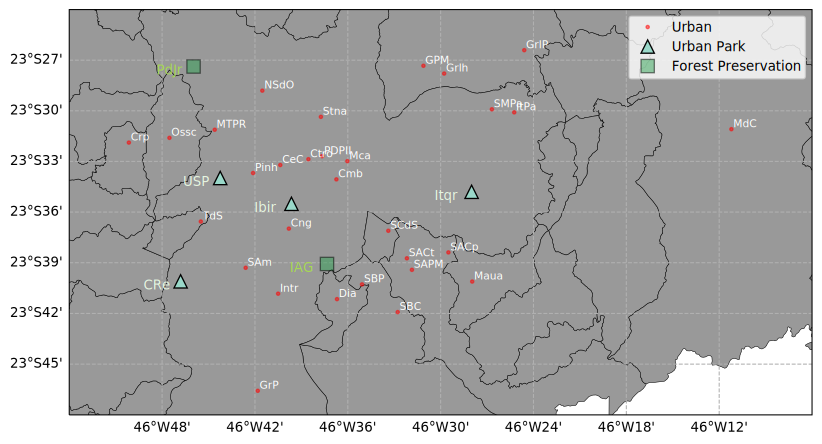
\includegraphics[width=1\textwidth]{fig/MASP_stations.pdf}
  		\caption{Air quality and meteorological stations network}

  		{\scriptsize Note:\\ The MASP map is in gray color. All stations except IAG belong to CETESB.}
  		\label{fig:mapStations}
	\end{figure}
	
  	\begin{figure}[htb]
		\includegraphics[width=1\textwidth]{fig/Stations_type_reduced.pdf}
  		\caption{Station classification type based on location in the S\~{a}o Paulo State. Maps Data: Google \copyright 2020, Maxar Technologies.}
  		\label{fig:station_types}
	\end{figure}
	
  \subsection{Air quality data}
  The period from 2014 to 2018 was analyzed, as shown in Figures~\ref{fig:Data} and \ref{fig:o3_years}.
  September and October presented higher hourly monthly mean surface ozone concentrations in many station types (e.g., Industry, Regional urban, Urban), as shown in Figure~\ref{fig:o3_time}.
  September presented more frequently higher surfer ozone concentrations than the other months and, for that reason, it can be considered the worst-case scenario.
  The maximum ozone concentration was reached at 15 hours (local time) in many station types (e.g., Forest preservation, Industry, Regional urban, and Urban).
  After 15 hours, during the evening, mean ozone concentrations decrease more than those recorded for December and January, as shown in Figure~\ref{fig:o3_time}.
  
  Regarding the interactions between surface ozone with other pollutants (CO, NO$_x$), Figure~\ref{fig:aqHour} shows charts by station type as hourly mean concentration based on data collected from September and October, 2018.
	The surface ozone reached its maximum levels between 14:00-15:00 hours (local time).
	CO and NO$_x$ (NO and NO$_2$) highest concentrations occurred at early morning (7:00-10:00 h) and evening (18:00-20:00 h) hours, positively correlated with the temporal distribution of emissions for light-duty and heavy-duty vehicles (Figure~\ref{fig:temp_distr}).
	Reduction of these pollutant concentrations between 11:00-19:00 hours is related to photochemical reactions that enhance ozone formation.
	Nocturnal ozone maximum concentration occurred around three and six hours (local time).
	This behavior was mentioned by \citet{Carvalho2015}, and can be associated with atmospheric transport from vertical levels, as it is mentioned in \citet{Mazzoli2013} and \citet{Andrade2017}.
	
	As mentioned in \citet{CETESB2019}, few stations monitor some hydrocarbons such as Benzene and Toluene (Figure~\ref{fig:HC_obs}).
	The hourly analysis shows a reduction of these VOC during the photochemical activity as shown in Figure~\ref{fig:hc_all_hour}.
  
  \begin{table}
	\centering
	\caption{CETESB stations considered to monthly analysis \\based on five years (2014-2018)}
	\label{tab:sta_year}
	\begin{tabular}{ll}
	\toprule
 	            Type &            Station \\
	\midrule
 Forest preservation &    Pico do Jaraguá \\
            Industry &           Paulínia \\
      Regional urban &  Campinas-Taquaral \\
      Regional urban &           Sorocaba \\
               Urban &         Interlagos \\
               Urban &        Carapicuíba \\
               Urban &  Parque D.Pedro II \\
               Urban &          Pinheiros \\
          Urban park &         Ibirapuera \\
          Urban park &           Itaquera \\
	\bottomrule
	\end{tabular}
   \end{table}
  
	
	\begin{figure}[!htb]
		\begin{center}
			\includegraphics[width=0.6\textwidth]{fig/aqHourSep_Urban.pdf}
			\includegraphics[width=0.6\textwidth]{fig/aqHourSep_Urban park.pdf}
			\includegraphics[width=0.6\textwidth]{fig/aqHourSep_Forest preservation.pdf}
		\end{center}
		\caption{Hourly mean concentrations for surface ozone (O$_3$), nitrogen monoxide (NO), nitrogen dioxide (NO$_2$), and carbon monoxide (CO) by station type in the MASP.}
		{\scriptsize Note. Shaded area corresponds to the standard deviation. }
		\label{fig:aqHour}
	\end{figure}
	
	\begin{figure}[hbt]
		\begin{center}
			\includegraphics{fig/byhour_all_polls.pdf}
		\end{center}
  		\caption{Hourly mean concentration by month (Sep-Oct, 2018), based on measurements in Pinheiros and S. André-Capuava stations.\\}
  		{\scriptsize Note: Toluene (Tol). Benzene (Ben). Shaded area corresponds to ozone concentration standard deviation.}
  		\label{fig:hc_all_hour}
	\end{figure}

  
  \subsection{Meteorological data}
  CETESB stations register hourly values for meteorological parameters such as surface temperature, relative humidity, wind speed and direction.
  However, these stations do not register hourly precipitation.
  Complementary, hourly data registered from the IAG climatological station in Água Funda was used for this study to compare with WRF-Chem model results.
  This data was requested on the IAG/USP station website: \\ \url{http://www.estacao.iag.usp.br/sol_dados.php}.\\
  The data was received as Excel files (hourly in rows and day in columns) and ordered as time series in rows and meteorological parameters in columns.
  Figure~\ref{fig:met_iag} in Appendix shows hourly time variation for September and October 2018 for eight meteorological parameters.
  Figure~\ref{fig:rain_cc_iag} in Appendix shows total daily rain and mean cloud cover; which in September (107 mm) was less than October (152 mm).
  According to \citet{Carvalho2015}, the weather condition in spring enhances ozone formation and is related to low cloud cover.
  September presented less values of cloud cover favoring the ozone formation due to photochemical activity.
  
  \section{Model performance evaluation}
  As recommended by \citet{Seinfeld2016}, three different performance index can be used to analyze the urban ozone models in the ability to reproduce the peak ozone concentrations, described below:
  
  \begin{itemize}
  	\item Analysis of predictions and observations paired in space and time.
  	\item Comparison of predicted and observed maximum concentrations.
  	\item Comparisons paired in space but not in time.
  \end{itemize}
  
Other recommendations are to use charts, plots, and statistical metrics for evaluating model results, letting us understand the model performance and its behavior, as suggested by \citet{Emery2017}.
  There are recommendations about statistics and benchmarks to assess photochemical model performance.
  \citet{Emery2017} analyzed statistical benchmarks applied to North American.
  For ozone, they recommended calculating statistics over temporal scales of one week (an episode), not longer than one month, and compared with recommended goals\footnote{"The more restrictive goals around the 33rd percentiles indicate statistical values that about one-third of top performing past applications in many U.S. modeling studies have met, and should be viewed as the best a model can be expected to achieve" \citep[defined in][]{Emery2017}.} and criteria\footnote{"The less restrictive criteria around the 67th percentile indicate statistical values that about two-thirds of past applications have met, and should viewed as establishing historical context that a majority of models have achieved" \citep[defined in][]{Emery2017}.} benchmarks shown in Table~\ref{tab:ozone_bench}.
  Although these statistical benchmarks were based on  North American modeling studies, \citet{Emery2017} recommendations are relevant to any such applications of state-of-science photochemical models.
  Therefore, they can be used for Brazil.
  In case one or two did not comply with the recommended criteria for Normalized Mean Bias (NMB), Normalized Mean Error (NME), or Pearson correlation coefficient (\textit{r}), the modeling application should not be considered "failure" \citep{Emery2017}.
  The same authors recommend to restrict periods when observations exceed a minimum threshold value ("cutoff"), particularly for ozone. As conclusion in the paper published by \citet{Emery2017}, they recommend:
  
  \begin{quote}
  	"applying a cutoff value of 40 ppb (observations) when calculating only NMB and NME for 1 hour ozone, for several physical and regulatory reasons beyond the need for statistical stability, but not for correlation as it is best characterized over the entire concentration distribution. The choice of 40 ppb is not absolute and should consider the chemical climatology of the region being modeled."
  \end{quote}
  
  On the other hand, even when the primary aim of this study is to understand ozone formation, it is also essential to consider meteorological conditions.
  Why do we need to evaluate meteorological results?  \citet{Emery2017} and \citet{Monk2019} suggest that it is essential due to its crucial role in the air quality simulations (e.g., ozone) since weather conditions are also a significant air quality driver.
  
  For this study, model results for September and October 2018 were compared with hourly measured data at each station.
  This evaluation let us to compare the analysis of modeled and observed values in space and time, suggested by \citet{Seinfeld2016}.
  Previously, units concentrations from model results (excluding CO) were converted from mixing ratio ppm(v) to $\mu$g~m$^{-3}$, using the following equation \citep{Seinfeld2016}:
  
  \begin{equation}
	Concentration ~[\mu g/m^3] = \frac{p ~M_i}{8.314~ T}\times \zeta _i ~[ppm] \label{eq:conv}
 \end{equation}
  
  Where $p$ is the atmospheric pressure in Pa (N~m$^{-2}$), M$_i$ is a molecular mass (g~mol$^{-1}$), $T$ is in Kelvin, and $\zeta _i$ is the mixing ratio in ppm, considering a molecular gas constant ($R$) equals to 8.1314 J K$^{-1}$~mol$^{-1}$ or Pa~m$^{-3}$~K$^{-1}$~mol$^{-1}$.
  Meteorological simulations of temperature and atmospheric pressure were used to convert concentration from ppm to $\mu$g~m$^{-3}$.
  
   The analysis of surface ozone was performed in two forms: 1-hr time series and the maximum daily 8-hr rolling mean (MDA8).
   Thus, the comparison of predicted and observed maximum concentrations is made based on MDA8 values for ozone concentrations through time plots by station types.
  Other pollutants as nitrogen oxides (NO, NO$_2$), CO, and toluene were also analyzed in time and space.
  We analyzed toluene only for some stations where it was measured during September and October 2018 period. 
  It is important to remark that the WRF-Chem model did not include benzene in the results.
  Therefore, it is excluded from the statistical analysis and the comparison with observations.
 
  Regarding meteorological evaluation, S\~{a}o Paulo state can be considered as a complex terrain due to areas with high altitudes (e.g., Pico do Jaragu\'{a}) and high buildings in the MASP.
  For this reason, meteorology model results were evaluated using specific statistical benchmarks suggested by \citet{Monk2019} for complex terrain (Table~\ref{tab:met_bench}).
  
  \begin{table}
	\centering
	\caption{Statistical benchmarks for surface ozone (1-hr or MDA8) \\ suggested by \citet{Emery2017}}
	\label{tab:ozone_bench}
	\begin{tabular}{lll}
  		\toprule
  		Statistical metric & Goal & Criteria \\
  		\midrule
  		NMB 	& <$\pm$5 \% 	& < $\pm$15 \% \\
  		NME    	& <15 \%		& < 25 \% \\
  		r		& > 0.75 \% 		& > 0.5 \% \\
  		\bottomrule
  		\multicolumn{3}{l}{\footnotesize Notes. Normalized Mean Bias (NMB), Normalized}\\
  		\multicolumn{3}{l}{\footnotesize Mean Error (NME), correlation coefficient (r).}
	\end{tabular}
 \end{table}
  
  \begin{table}
	\centering
	\caption{Statistical benchmarks for meteorology parameters suggested by \citet{Monk2019}}
	\label{tab:met_bench}
	\begin{tabular}{lll}
	\toprule
  	Parameter & Statistical metric & Complex terrain \\
 	 \midrule
  	Temperature [K]			& MAGE &  $\leq$ 3 \\
  		  					& MB   &  $\leq \pm$1\\
  	      					& IOA  &  $\geq$ 0.8 \\ 
  	Relative humidity   		& MAGE & < 20 \% \\
  							& MB   & < $\pm$10 \%\\
  							& IOA  &  $\geq$ 0.6\\
  	Wind speed [ms$^{-1}$]	& RMSE & $\leq$ 2.5\\
  							& MB   & $\leq \pm$1.5 \\
  							& IOA  & $\geq$ 0.6\\
  	Wind direction [degree] & MAGE & $\leq$ 55	\\
  							& MB   & $\leq \pm$10  \\
  	\bottomrule
  	\multicolumn{3}{l}{\footnotesize Notes. Mean Absolute Gross Error (MAGE), Mean Bian (MB), }\\
  	\multicolumn{3}{l}{\footnotesize index of agreement (IOA), Root Mean Square Error (RMSE).}
  	\end{tabular}
\end{table}

More details, such as utilities, can be found in Appendix~\ref{ap04}. Statistic equations are described as follows based on the description by \citet{Emery2017}:
  
  \begin{align}
  MAGE =&~ \frac{1}{N}\sum|P_j - O_j| \\
  MB = &~  \frac{1}{N}\sum(P_j - O_j)\\
  IOA = &~ 1 - \frac{\sum(P_j-O_j)^2}{\sum(|P_j+\overline{O}|+|O_j+\overline{O}|)^2}\\
  NMB =&~ \frac{\sum(P_j-O_j)}{\sum O_j}\times 100\\
  NME =&~ \frac{\sum|P_j-O_j|}{\sum O_j}\times 100\\
  r =&~ \frac{\sum[(P_j-\overline{P})\times(O_j-\overline{O})]}{\sqrt{\sum(P_j-\overline{P})^2\times \sum(O_j-\overline{O})^2}}
  \end{align} 
    
  \subsection{Hypothesis test for Pearson's r}
 The correlation coefficient (\textit{r}) gives us information about how two datasets have a linear relationship or not.
  A positive perfect correlation (+1) corresponds to all the pairs lying on a straight line with a positive slope when a scatter diagram is used.
  It is desired to achieve in air quality modeling (a perfect model!). 
  However, a few paired values could generate errors for the correlation coefficient, which could not be robust or significant.
  Significance and confidence interval can be calculated for correlation coefficient based on t-test (two-tailed).
  %, available in the Python function \verb|r_pearson_sign| as part of \verb|mod_stats.py| script.
   Based on \citet{Navidi2019} t-test statistical evaluation methodology, we defined Null (H$_o$) and Alternative hypothesis (H$_A$), considering an alpha ($\alpha$) equals to 0.05 for degree freedom (df) equals to n-2, where n is the number of paired values:
  \begin{itemize}
  	\item H$_o$: $\rho$ = 0 (samplings of x (obs) and y (mod) are not correlated)
  	\item H$_A$: $\rho$ $\neq$ 0
  \end{itemize}
  Where $\rho$ denotes the population correlation between x and y.
  Then, assuming that H$_o$ is true, a statistical test is computed and used to asses the strength of the evidence against H$_o$.
  Also, we compute the P-value of the test that is the probability and is also called the \textbf{observed significance level}.
  The P-value measures the plausibility of H$_o$.
  So, if the P-value is sufficiently small, we may be willing to abandon the assumption that H$_o$ is true and believe H$_A$ instead (rejecting the null hypothesis).
  As a practical rule, if the t critical value (calculated from $\alpha$=0.05 and n-2 degree freedom) is less than the t-statistic, we will reject the null hypothesis and accept the H$_A$.
  Therefore, we can state "there is enough evidence to conclude that there is a significant linear relationship between x (obs) and y (mod) because the correlation coefficient is significantly different from zero."
  The formula for the t-statistic value calculation is \citep{Navidi2019}:
  
  \begin{align}
  	t = \frac{r\sqrt{n-2}}{\sqrt{1-r^2}}
  \end{align}
  
  Where r is the sample correlation of the n points. 
  The t-statistic value has the same sign as the correlation coefficient.






  
  
  
		\chapter{\bf Results and Discussion}\label{chap:resul}
\epigraph{\textit{Assure me that I yet may change these shadows you have shown me.}}{Charles Dickens, \textit{A Christmas Carol}}
   \noindent  This chapter presents the emission inventory results for September and October of 2018 and WRF-Chem model results for the second modeling domain ($\delta$X = 3 km) for all scenarios.
   Two scenarios (RCP 4.5 and RCP~8.5 for 2030) are future predictions oddly reminiscent of Dickens.
      
   In Section~\ref{sec:res_curr}, this study evaluates the WRF-Chem model results for the current conditions (September and October 2018 period) based on the meteorological IC/BC, emission for anthropogenic (road transport, industry, and residential), and biogenic sources.
   
   Statistical evaluation for surface ozone simulations covers detailed analyses for the global data, station types, and station locations.
   Further analyses show variations for some ozone precursors (NO$_x$, CO, and toluene) by hour of day as an average for the all analyzed period (i.e., Pinheiros station).
   
   In Section~\ref{sec:res_fut}, future meteorological conditions and surface ozone concentrations from the WRF-Chem model are presented. 
   These results are based on the same emission rates used to evaluate the model for current conditions, with the change for meteorological IC/BC provided from the CESM1 datasets: RCP 4.5 and RCP~8.5 scenarios; representing a set of possible humankind future pathways based on GHG emissions, air pollutants concentrations, and land use/land cover changes.   
   
   \section{Evaluation results for current conditions}\label{sec:res_curr}
   % First specific objective: prepare and update the emission file for the year 2018, representative of the modeling domain areas for the São Paulo state.
    
  \subsection{Anthropogenic emissions}\label{subsec:res_anth}
   This section shows the spatial and temporal anthropogenic emissions distribution.
   The results are based on emissions inventory approaches from the bottom-up methodology for the road transport sector \citep{Andrade2015} and from the EDGAR-HTAP datasets \citep{Janssens2015} interpolation in space and time using the anthro\_emiss emission pre-processor \citep{Kumar2020} for the industrial and residential sectors.
   
   We tested 11 experiments, running the model for seven\footnote{Two first days are spin-up, not included in the analysis.} non-rainy days based on different emission files, the base emission and some pollutants with a correction factor.
   Considering \citet{Emery2017} benchmarks, experiment 10 with a correction factor of 0.8 for NO$_x$ road transport emission files represented better the ozone formation in the MASP for September and October 2018.
   However, these tests showed the difficulty of improving other pollutants' simulations (NO$_x$, CO, and toluene) when compared with observations. 
   The emission files are the primary error source for simulations and require to be corrected as many works have reported for São Paulo and other cities outside of Brazil \citep{Russell2000, Holnicki2015, Andrade2017, Ibarra2020}.
   Vehicular emissions \citep[described in][]{Andrade2015} have limitations on the spatial and temporal distribution (e.g., roads only for heavy-duty vehicles), even when considering a bottom-up approach.
   
	Figure~\ref{fig:anth_dist}, as for instance, shows the spatial distribution of NO emissions for the second modeling domain.
	Based on CBM-Z chemical mechanism, 21  species of emission rates were considered in WRF-Chem emission files (i.e., \verb|wrfchemi_{00z, 12z}_{d01, d02}|).
	Figure \ref{fig:emiss_temp} shows emission rates and the temporal distribution of Industry, Residential, and Road Transport sectors. 
	Only road transport emissions present a temporal distribution based on information available in \citet{Andrade2015} (Figure~\ref{fig:temp_distr}).
	Table~\ref{tab:emi_d02} shows emission rates in units of kilo-tonnes per year (kt/year) accumulated in the second domain, based on the calculated emissions for the period September 2018.
	
	\begin{figure}[htb]
		\begin{center}
			\includegraphics[width=.9\textwidth]{fig/E_NO_emi_d02.pdf}
		\end{center}
  		\caption{NO emissions for second modeling domain in SE Brazil}
  		{\scriptsize Note:\\ Only Total emission files were used as input to the WRF-Chem model. Anthropogenic emissions were summed using a Python script \verb|wrfchemi.py|. LT= Local Time. X and Y axis labels are in  local coordinates.}
  		\label{fig:anth_dist}
	\end{figure}
	
	\begin{figure}[htpb]
		\centering
		\includegraphics[width=.8\textwidth]{fig/emi_kt.pdf}
		\includegraphics[width=.8\textwidth]{fig/emi_NO_time_kt.pdf}
  		\caption{Emission rates by species (part a) and temporal distribution (part b) for all days for NO emission rates and by sector}	
  		\label{fig:emiss_temp}
	\end{figure}
	
	\begin{table}
\centering
\caption{Emission rates (kt/year) for the second modeling domain based on activity data for the September 2018 period}
\label{tab:emi_d02}
\begin{tabular}{llrrr}
\toprule
{} &            ID &     Road &  Industrial &  Residential \\
Species                    &               &          &             &              \\
\midrule
Carbon monoxide            &            CO &  1412.29 &      510.65 &       191.80 \\
Nitrogen oxide             &            NO &   244.23 &      134.21 &         7.59 \\
Nitrogen dioxide           &        NO$_2$ &    27.14 &       22.87 &         1.29 \\
Nitrogen oxides            &        NO$_x$ &   271.37 &      157.08 &         8.88 \\
Sulfur dioxide             &        SO$_2$ &    30.74 &      133.09 &        12.92 \\
Ammonia                    &        NH$_3$ &     4.71 &       21.41 &         0.13 \\
Isoprene                   &           ISO &     0.52 &        0.00 &         0.00 \\
Ethane                     &           ETH &     8.31 &        6.53 &         0.73 \\
Propane                    &           HC3 &    52.41 &       39.19 &         4.39 \\
Alkanes (k$_{OH}$ 0.5 - 1) &           HC5 &    79.96 &       45.73 &         5.12 \\
Alkanes (k$_{OH}$ 1 - 2)   &           HC8 &   126.25 &       45.73 &         5.12 \\
Xylenes                    &           XYL &    55.87 &       19.60 &         2.19 \\
Alkenes (internal)         &           OL2 &    41.90 &       52.26 &         5.85 \\
Alkenes (terminal)         &           OLT &    75.85 &       45.73 &         5.12 \\
Alkenes (primary)          &           OLI &    48.41 &       26.13 &         2.92 \\
Toluene                    &           TOL &    80.50 &       26.13 &         2.92 \\
Formaldehyde               &          HCHO &    28.17 &       32.66 &         3.66 \\
Aldehydes                  &           ALD &    38.17 &       26.13 &         2.92 \\
Ketones                    &           KET &     0.45 &        0.00 &         0.00 \\
Methanol                   &      CH$_3$OH &     0.56 &        0.00 &         0.00 \\
Ethanol                    &  C$_2$H$_5$OH &   396.17 &      287.42 &        32.17 \\
\bottomrule
\end{tabular}
\end{table}




	
  \subsection{Meteorological model evaluation}\label{subsec:res_met}
  WRF-Chem model results were compared with measurements from CETESB stations network and the IAG/USP climatological station located in Água Funda.
The meteorological parameters extracted from the model for the statistical evaluation were 2-m temperature [$^\circ$C], 2-m relative humidity [\%], accumulated rain ($rainc$ and $rainnc$) [mm], wind speed [ms$^{-1}$] and direction [degree] at 10 m above the ground.

  Model simulations at IAG/USP location were analyzed. 
  This station complies with the World Meteorological Organization standards to locate a weather station \citep{WMO2018}.
  Furthermore, this station recorded the hourly rainfall rate, a parameter not recorded by the CETESB stations network.
  
  \subsubsection{IAG/USP climatological station}
Figure~\ref{fig:met_iag_comp} shows comparison between model simulations and observed values for each meteorological parameter, such as temperature, relative humidity, rain rate, wind speed, and wind direction.
Tables~\ref{tab:stats_iag} and \ref{tab: r_sign_iag} show statistical model evaluation results and t-test values for correlation coefficient for the IAG/USP station.

\begin{figure}[!hbt]
  \includegraphics[width=1\textwidth]{fig/met_IAG_comparison}
  \caption{Comparison between observed and modeled values for meteorological parameters for the IAG/USP station during the period Sep-Oct 2018}
  \label{fig:met_iag_comp}
\end{figure}

Temperature model results comply with MAGE and IOA statistical benchmarks suggested by \citet{Monk2019} for complex terrain.
However, MB result is not less than 1 ºC.
There is an overprediction of +1.56 ºC on average compared with observations.

Relative humidity from model results comply with the three statistical benchmarks (MAGE and MB units are in \%, apply for the MASP).
Thus, model results presented high accuracy to simulate this meteorological parameter.

Wind speed model results comply with the RMSE statistical benchmark, but not for the others (MB and IOA).
The model over-predicted in +1.69 m/s the average wind speed observations.
Wind direction model results comply with statistical benchmarks for MAGE (value less than 55) and MB (value less than 10).
Thus, the model has a good capability to simulate wind directions at IAG/USP station.
Figure~\ref{fig:wrplot_iag} shows the two wind rose plots, one with the modeled values and the other for the observation values. The frequency of calm winds is greater in observations than in the model results.

\begin{figure}[!hbt]
  \centering
  \includegraphics{fig/WRplot_IAG_sep_oct2018}
  \caption{Wind rose plot for Sep-Oct 2018 period at the IAG/USP station, for modeled and observed values. Wind speed simulations less than 0.5 m/s were replaced by 0 m/s to compare with observations.}
  \label{fig:wrplot_iag}
\end{figure}

Statistical results for rain simulations presented low performance, so the model was not accurate to represent rain observations recorded at the IAG/USP station.
However, the hypothesis t-test suggests that there is a significant linear relationship between modeled and observed values based on t-critical being less than the t-statistic value (Table~\ref{tab: r_sign_iag}).
Despite a low correlation, the rainfall simulation values have significant statistical indexes with the observations. 
Figure~\ref{fig:iag_daily_rain} shows comparisons between modeled and observed values for total daily rain with reasonable accuracy for September 14 and October 24, 2018.

\begin{figure}[!hbt]
	\centering
  \includegraphics[width=.8\textwidth]{fig/iag_daily_rain}
  \caption{Comparison between observed and modeled values for total daily rain rate during Sep-Oct 2018 for the IAG/USP station}
  \label{fig:iag_daily_rain}
\end{figure}

\begin{table}
\centering
\begin{threeparttable}
\caption{Statistical results for meteorological parameters for Sep-Oct 2018 (IAG/USP station)}
\label{tab:stats_iag}
\begin{tabular}{lrrrrr}
\toprule
Statistic\tnote{(a)} & 2-m Temp. ($^{\circ}$C) & 2-m RH (\%) & Rain rate (mm)  & W. Speed (m~s$^{-1}$) & W. Dir. ($^{\circ}$)  \\
\midrule
n      &  1461.00 &  1461.00 &  1461.00 &  1461.00 &  1461.00 \\
MB     &     1.56 &    -9.00 &     0.13 &     1.69 &     5.02 \\
MAGE   &     1.97 &    11.15 &     0.42 &     1.84 &    32.57 \\
RMSE   &     2.66 &    14.66 &     1.72 &     2.22 &        - \\
IOA    &     0.89 &     0.78 &     0.23 &     0.43 &        - \\
r      &     0.85 &     0.71 &     0.11 &     0.37 &        - \\
Mm     &    20.32 &    74.30 &     0.30 &     3.37 &        - \\
Om     &    18.76 &    83.30 &     0.18 &     1.69 &        - \\
Msd    &     3.96 &    15.68 &     1.20 &     1.50 &        - \\
Osd    &     3.89 &    14.46 &     1.35 &     0.91 &        - \\
t-stat &    61.63 &    38.51 &     4.23 &    15.21 &        - \\
t-crit &     1.96 &     1.96 &     1.96 &     1.96 &        - \\
\bottomrule
\end{tabular}
\begin{tablenotes}
{\scriptsize
	\item[(a)] MB = Mean bias, MAGE = Mean Absolute Gross Error, RMSE = Root Mean Square Error, Mm = Mean of modeled values, Om = Mean of observed values, Msd = Standard deviation of modeled values, and Osd = Standard deviation of observed values. Units depend on the meteorological parameter. Correlation coefficient (r) is in dimensionless units. Statistical parameters are t-test statistical (t-stat) and t critical (t-crit).}
\end{tablenotes}
\end{threeparttable}
\end{table}


\begin{table}
\centering
\caption{Correlation t-test values by meteorological parameter for Sep-Oct 2018 (IAG/USP station)}
\label{tab: r_sign_iag}
\begin{tabular}{lrrrr}
\toprule
{} &  2-m Temp. &   2-m RH &  W. Speed &  Rain rate \\
\midrule
t-statistic &  61.63 &  38.51 &  15.21 &  4.23 \\
t-critical  &   1.96 &   1.96 &   1.96 &  1.96 \\
\bottomrule
\end{tabular}
\end{table}



\subsubsection{CETESB and IAG/USP grouped by station types}
Statistical results considered all stations with non missing values for temperature, relative humidity, wind speed, and wind direction.
Table~\ref{tab:stats_all} shows global statistical results for each meteorological parameter.

\begin{table}[ht]
\centering
\caption{Statistical results for meteorological parameters for Sep-Oct 2018 (all stations)}
\label{tab:stats_all}
\begin{tabular}{lrrrrrrrrrr}
\toprule
{} &      n &     MB &   MAGE &   RMSE &   IOA &     r &     Mm &     Om &    Msd &    Osd \\
\midrule
2-m Temp. ($^{\circ}$C) 	&  38727 &   1.30 &   1.94 &   2.54 &  0.92 &  0.89 &  21.99 &  20.69 &   4.36 &   4.74 \\
2-m RH (\%)				&  37298 &  -7.32 &  11.18 &  14.46 &  0.84 &  0.76 &  68.87 &  76.19 &  17.71 &  18.49 \\
W. Speed (m~s$^{-1}$) 	&  45412 &   1.38 &   1.71 &   2.13 &  0.52 &  0.39 &   3.36 &   1.98 &   1.70 &   1.12 \\
W. Dir. ($^{\circ}$) 	&  43189 & -21.66 &  50.58 &      - &     - &     - &      - &      - &      - &      - \\
\bottomrule

\end{tabular}
\end{table}


Model results for temperature comply with two statistical benchmark (MAGE and IOA).
The model over-predicted temperature results with +1.31 ºC based on modeled (Mm) and observed (Om) mean values, also shown as MB result in Table~\ref{tab:stats_all}.

In general terms, the model has a good performance for relative humidity because simulations comply with all the benchmarks (MAGE < 20\%, MB < $\pm$ 10\%, and IOA $\geq$ 0.6).
However, simulations under-predicted measurements as we can see in the negative MB value.

Model simulations for wind speed comply with two (RMSE and MB) of three statistical benchmarks.
The IOA value does not reach the statistical benchmark ($\geq$ 0.6).
Regarding to wind direction, only one statistical value (MAGE) complies with the benchmark ($\leq$ 55).
The MB (as absolute value) for wind direction is greater than the statistical benchmark ($\leq~$10).

Considering correlation results, Table~\ref{tab: r_sign_met_all} shows t-test values and number of samplers (n) analyzed; which indicate a significant linear relationship between modeled and observed values due to t-statistic values are greater than t-critical values.

\begin{table}
\centering
\caption{Correlation t-test values by meteorological parameter for Sep-Oct 2018 (all stations)}
\label{tab: r_sign_met_all}
\begin{tabular}{lrrr}
\toprule
{} &     2-m Temp. (ºC) &  2-m RH (\%) &  W. Speed (m~s$^{-1}$) \\
\midrule
t-statistic &    390.21 &     236.90 &     94.53 \\
t-critical  &      1.96 &       1.96 &      1.96 \\
n           &  39966.00 &   38538.00 &  46920.00 \\
\bottomrule
\end{tabular}
\end{table}



Further specific analysis by station type are shown in Appendix Table~\ref{tab:stats_all_type}, and summarized in Table~\ref{tab:sum_bench}, which shows model performance results for each meteorological parameter and station type.
The WRF-Chem model has a good performance for the relative humidity simulations.
Figure~\ref{fig:rh_cetesb} in Appendix shows time series as a daily mean for relative humidity, where model results and observations are compared by station type. 
Temperature model results comply with two of three statistical benchmarks.
Figure~\ref{fig:temp_cetesb} in Appendix shows temperature values as a daily mean for model results compared with observations by each station type.
Only model results for "Industry station type" presented good performance.

Finally, the wind was difficult to simulate and did not present good results compared with observed values.
Statistical results suggest low capability of the model to simulate wind speed in urban and forest areas (i.e., Pico do Jaraguá station).
However, this is not particularly surprising given that CETESB stations aim to measure air quality parameters, and many stations could not comply with WMO recommendations to install weather station \citep{WMO2018}.
Furthermore, there are errors in the model due to low resolution to represent the topography, such as hills in the higher terrain (i.e., Pico do Jaraguá). 
Figure~\ref{fig:ws_cetesb} in Appendix shows wind speed values as a daily mean for model results and observations; modeling values belonging to "Forest preservation sites" highly overpredicted observed values more than other station types.

\begin{table}
\centering
\caption{Summary of compliance of statistical benchmarks }
\label{tab:sum_bench}
\begin{tabular}{lrrrrrr}
\toprule
{}        &    Urban &  U. park &  R. urban &    Ind. &  F. pre. & \\
\midrule
2-m Temp. ($^{\circ}$C)  (3 benchmarks)   &    $\checkmark$$\checkmark$ &  $\checkmark$$\checkmark$ &    $\checkmark$$\checkmark$ &  $\checkmark$$\checkmark$$\checkmark$ &    $\checkmark$$\checkmark$ & 11 \\
2-m RH (3 benchmarks)  &     $\checkmark$$\checkmark$$\checkmark$ &   $\checkmark$$\checkmark$ &     $\checkmark$$\checkmark$$\checkmark$ &   $\checkmark$$\checkmark$$\checkmark$ &     $\checkmark$$\checkmark$$\checkmark$ & 14\\
W. Speed (m s$^{-1}$) (3 benchmarks) &     $\checkmark$$\checkmark$ &   $\checkmark$ &     $\checkmark$$\checkmark$ &   $\checkmark$ &   & 6  \\
W. Dir. ($^{\circ}$) (2 benchmarks)  &     $\checkmark$ &   $\checkmark$$\checkmark$ &      &   $\checkmark$ &     $\checkmark$ & 5\\
\bottomrule
 & 8 & 7 & 7 & 8 & 6\\
\end{tabular}
\end{table}
	
  \subsection{Air quality model evaluation} \label{subsec:res_aq}
  This section shows the model output for current conditions (Sep. and Oct. 2018), their evaluation through statistical analysis, and the comparison between model simulations and observations from CETESB air quality stations network.
  The parameters extracted from the model for the statistical evaluation were nitrogen monoxide (NO in $\mu$g~m$^{-3}$), nitrogen dioxide (NO$_2$ in $\mu$g~m$^{-3}$), carbon monoxide (CO in ppm), toluene ($\mu$g~m$^{-3}$), and surface ozone (O$_3$ in $\mu$g~m$^{-3}$).
   Ozone 8-hr rolling mean was also calculated from hourly time series for model simulated and observed values.
   Some stations located close to coastal zone were not included as part of statistical evaluation due to low performance of WRF-Chem model, which are:
   
   \begin{itemize}
   	\item Santos
   	\item Santos-Ponta da Praia
   	\item Cubat\~{a}o-Centro
   	\item Cubat\~{a}o-Vale do Mogi
   	\item Cubat\~{a}o-V. Parisi
   \end{itemize}
   
   Furthermore, model hourly simulations for September 14-15, 2018, were not considered in the statistical analysis due to cloud and rainfall conditions not represented appropriately by the WRF-Chem model.
   Figure~\ref{fig:rain_sep18} in Appendix shows mean cloud cover and total rain by day.
   Thus, 57 stations with hourly observations were compared with WRF-Chem model results, according to the station types (i.e., Forest Preservation, Urban, Urban Park, Regional Urban, and Industry).
   As highlighted in Figure~\ref{fig:mapStations}, the station types inside the MASP correspond to Forest Preservation, Urban, and Urban Park.

  Global statistical results in Table~\ref{tab: gl_st} show correlation coefficients (r) for ozone  above 0.50 that comply with the criteria level as statistical benchmark suggested by \citet{Emery2017}.
  Average values of NMB and NME for ozone comply with the goal level ($\leq\pm$5 \% for NMB) and criteria level ($\leq$25 \% for NME).
  Based on MB results, positive values are indicators that simulations are overestimating the observations.
  
  Primary pollutants (NO$_x$ and CO) have low values of correlation coefficients.
  On average, the model over-predicted NO$_2$ concentrations due to positive values for MB (+4.12 $\mu$g m$^{-3}$ for Sep. 2018) and NMB (15.69~\% for Sep. 2018).
  However, simulations for September 2018 period under-predicted NO and CO concentrations which NMB values are -6.39~\% and -52.3~\%, respectively.
  These underpredictions increase for October 2018 period with -48.06~\% and -61.77~\%, respectively.
  Probably, NO and CO emissions could be underestimated, mainly for the October 2018 period.
  The spatial distribution of NO$_x$ emission is subjected to errors, considering that heavy-duty vehicles in the MASP use specific roads where trucks are concentrated on motorways around the city \citep{Ibarra2020}.
  
  \begin{table}
\centering
\caption{Global statistical results for air quality parameter}
\label{tab: gl_st}
\begin{tabular}{lrrrrrrrrrr}
\toprule
{} & \multicolumn{5}{l}{Sep. 2018} & \multicolumn{5}{l}{Oct. 2018} \\
{} &        o3 &        no &       no2 &       nox &       co &        o3 &        no &       no2 &       nox &        co \\
\midrule
n     &  23921.00 &  21693.00 &  21693.00 &  21693.00 &  9837.00 &  26034.00 &  24099.00 &  24099.00 &  24099.00 &  12152.00 \\
MB    &      9.32 &     -0.55 &      4.09 &      3.54 &    -0.26 &     13.15 &     -4.10 &      1.39 &     -2.71 &     -0.31 \\
MAGE  &     24.01 &     10.50 &     18.33 &     27.75 &     0.29 &     22.51 &      8.73 &     15.44 &     22.99 &      0.33 \\
RMSE  &     30.07 &     23.78 &     25.77 &     43.63 &     0.40 &     29.43 &     21.89 &     21.79 &     37.44 &      0.44 \\
NMB   &     19.24 &     -6.54 &     15.56 &     10.20 &   -52.28 &     31.65 &    -47.84 &      5.92 &     -8.46 &    -61.76 \\
NME   &     49.57 &    124.67 &     69.75 &     79.99 &    59.26 &     54.17 &    101.81 &     65.74 &     71.70 &     64.64 \\
IOA   &      0.80 &      0.46 &      0.62 &      0.58 &     0.45 &      0.76 &      0.31 &      0.65 &      0.56 &      0.44 \\
r     &      0.67 &      0.25 &      0.39 &      0.34 &     0.19 &      0.64 &      0.16 &      0.42 &      0.34 &      0.17 \\
Mm    &     57.75 &      7.87 &     30.36 &     38.23 &     0.24 &     54.71 &      4.47 &     24.87 &     29.35 &      0.19 \\
Om    &     48.43 &      8.42 &     26.27 &     34.70 &     0.49 &     41.56 &      8.58 &     23.48 &     32.06 &      0.51 \\
Msd   &     37.75 &     17.50 &     25.47 &     38.68 &     0.12 &     33.27 &      8.57 &     20.81 &     26.71 &      0.08 \\
Osd   &     31.36 &     20.97 &     19.99 &     36.90 &     0.31 &     27.49 &     21.14 &     19.47 &     36.83 &      0.32 \\
NMB 2 &      2.24 &       NaN &       NaN &       NaN &      NaN &      1.92 &       NaN &       NaN &       NaN &       NaN \\
NME 2 &     21.66 &       NaN &       NaN &       NaN &      NaN &     20.80 &       NaN &       NaN &       NaN &       NaN \\
\bottomrule
\end{tabular}
\end{table}


  
   \subsubsection{Surface ozone}
  Ozone model results were also evaluated for each station type, as shown in Table~\ref{tab: o3_sta}. 
  Three statistical values (NMB, NME, and r) for many station types complied with at least the criteria level of benchmarks suggested by \citet{Emery2017}.
  NMB values for ozone are less than the range $\pm$15\% for those stations in the MASP.
  Only Forest preservation (F. pre.) and Urban park (U. park) stations comply with some statistical goal level of benchmarks, such as NMB (values <~$\pm$5\%) for September 2018 period.
  Only for stations classified as Industry (e.g., Santa Gertrudes), the correlation coefficient value for September 2018 complies with the goal level as a statistical benchmark (r >~0.75).
  Based on hypothesis t-test evaluation, there is a significant linear relationship between observed and simulated values because the correlation coefficient is significantly different from zero, as shown in Table~\ref{tab: r_sign} ($\alpha$ = 0.05 at confidence interval of 95~\%).
  We can see that t-statistic values are greater than t critical values, which mean P-values are sufficiently small to reject the null hypothesis and accept the alternative hypothesis: "there is enough evidence to reject the null hypothesis (H$_o$)".
  \begin{table}
\begin{threeparttable}[b]
\centering
\caption{Statistical results for surface ozone by station type}
\label{tab: o3_sta}
\begin{tabular}{lrrrrrrrrrr}
\toprule
Month & \multicolumn{5}{l}{Sep. 2018} & \multicolumn{5}{l}{Oct. 2018} \\
type &   F. pre. &       Urb &  U. park &     Ind &  R. urb. &   F. pre. &       Urb &  U. park &     Ind &  R. urb. \\
Statistic\tnote{(a)} \\
\midrule
n    &    636.00 &  11314.00 &  2205.00 &  637.00 &  9057.00 &    709.00 &  12383.00 &  2663.00 &  706.00 &  9500.00 \\
MB   &      0.51 &      4.03 &    -1.68 &   17.20 &    18.75 &      4.46 &     10.33 &     4.55 &   19.91 &    19.50 \\
MAGE &     24.44 &     23.27 &    23.35 &   27.23 &    24.83 &     22.11 &     21.25 &    21.03 &   28.69 &    24.11 \\
RMSE &     30.64 &     29.54 &    29.25 &   32.52 &    30.70 &     28.38 &     28.46 &    27.69 &   35.10 &    30.71 \\
NMB\tnote{(b)}  &      \textcolor{blue}{\bf 1.02} &      \textcolor{blue}{8.96} &    \textcolor{blue}{\bf -3.49} &   \textcolor{red}{33.95} &    \textcolor{red}{35.57} &     \textcolor{blue}{10.75} &     \textcolor{red}{27.77} &    \textcolor{blue}{11.52} &   \textcolor{red}{45.85} &    \textcolor{red}{40.85} \\
NME\tnote{(b)}  &     \textcolor{red}{48.90} &     \textcolor{red}{51.75} &    \textcolor{red}{48.54} &   \textcolor{red}{53.75} &    \textcolor{red}{47.11} &     \textcolor{red}{53.28} &     \textcolor{red}{57.12} &    \textcolor{red}{53.21} &   \textcolor{red}{66.05} &    \textcolor{red}{50.50} \\
\bf NMB\tnote{(c)} & \textcolor{blue}{7.19} & \textcolor{blue}{7.39} & \textcolor{blue}{\bf -0.58} & \textcolor{blue}{-7.26} &    \textcolor{blue}{\bf -0.28} &     \textcolor{blue}{\bf -4.48} &  \textcolor{blue}{8.97} &     \textcolor{blue}{\bf 4.75} &   \textcolor{blue}{-8.53} &    \textcolor{blue}{\bf -1.87} \\
\bf NME\tnote{(c)} & \textcolor{red}{30.59} &     \textcolor{blue}{24.75} &    \textcolor{blue}{22.67} &   \textcolor{blue}{17.46} &    \textcolor{blue}{19.22} &     \textcolor{blue}{24.36} &     \textcolor{blue}{23.26} &    \textcolor{blue}{23.02} &   \textcolor{blue}{20.63} &    \textcolor{blue}{18.57} \\
IOA  &      0.81 &      0.80 &     0.82 &    0.85 &     0.76 &      0.74 &      0.77 &     0.80 &    0.76 &     0.69 \\
\bf r   &      \textcolor{blue}{0.72} &      \textcolor{blue}{0.68} &     \textcolor{blue}{0.69} &    \textcolor{blue}{\bf 0.80} &     \textcolor{blue}{0.69} &      \textcolor{blue}{0.60} &      \textcolor{blue}{0.66} &     \textcolor{blue}{0.67} &    \textcolor{blue}{0.69} &     \textcolor{blue}{0.60} \\
Mm   &     50.49 &     49.00 &    46.43 &   67.85 &    71.45 &     45.97 &     47.52 &    44.07 &   63.34 &    67.25 \\
Om   &     49.98 &     44.97 &    48.11 &   50.65 &    52.70 &     41.51 &     37.20 &    39.52 &   43.43 &    47.74 \\
Msd  &     43.91 &     39.91 &    40.11 &   36.60 &    28.55 &     34.73 &     34.90 &    36.53 &   30.54 &    25.17 \\
Osd  &     28.98 &     28.95 &    31.62 &   46.19 &    32.56 &     24.68 &     25.90 &    27.90 &   39.49 &    27.37 \\
\bottomrule
\end{tabular}
\begin{tablenotes}
{\scriptsize
	\item[(a)] MB, MAGE, RMSE, Mm, Om, Msd, and Osd values are in $\mu$g~m$^{-3}$. Correlation coefficient is in dimensionless units.
	\item[(b)] No cutoff was applied.
	\item[(c)] A cutoff value of 80 $\mu$g~m$^{-3}$ was applied to calculate NMB and NME only for 1-hr ozone, suggested by \citet{Emery2017}. Units are in percentage. Units are in percentage. Values in bold blue comply with the Goal benchmark and in only blue with the Criteria benchmark for ozone. Values in red don't comply with the statistical benchmarks.}
\end{tablenotes}
\end{threeparttable}
\end{table}


  \begin{table}
\centering
\caption{t-test values for correlation coefficient (r) for Sep. 2018}
\label{tab: r_sign}
\begin{tabular}{lrrrrr}
\toprule
{} &  F. pre. &    Urb &  U. park &    Ind &  R. urb. \\
\midrule
t-statistic &    26.21 &  98.94 &    44.87 &  33.70 &    91.00 \\
t critical  &     1.96 &   1.96 &     1.96 &   1.96 &     1.96 \\
\bottomrule
\end{tabular}
\end{table}
  
 Based on the score shown in \ref{tab:bench_o3}, both months presented a better performance of simulations for ozone. 
Stations belonging to the MASP comply with two of three statistical benchmarks, as shown in Table \ref{tab:bench_o3}.
 Despite of cloudy and rain conditions, simulations for October 2018 presented good performance as September 2018.
  Likewise, the cold front system reached the MASP for six days during October 5-10, 2018, according to the \textit{Centro de Hidrografia da Marinha} \citep{CHM2020}.
  As was mentioned at the beginning of this chapter, the WRF-Chem model, due to its configuration, could not simulate adequately heavy rainy days and consequently their influence in the ozone formation.
  Furthermore, the model performance evaluation (Table \ref{tab:bench_o3}) revealed that surface ozone simulations presented better values for station types as `Forest preservation' (only for October), `Urban park', `Industry' (only for September), and `Regional urban'.
  A possible explanation for the low performance attributed to Urban stations could be related to the model resolution, in which spatial emission rates distribution (3 km $\times$ 3 km) do not represent local emission for stations closer to main roads.
  
\begin{table}[b]
\centering
\caption{Summary of compliance of the ozone statistical benchmarks by station types}
\label{tab:bench_o3}
\begin{tabular}{lrrrrrrr}
\toprule
Month & Statistic        &   F. pre.	 &  Urban     &  U. park &   Ind   &  R. urb. & \\
\midrule
Sep. 2018 & NMB 		 &  \ok	     &  \ok       &  \ok \ok & \ok     & \ok \ok  & 7  \\
          & NME          &           &  \ok       &  \ok     & \ok     & \ok      & 4  \\
          & r            &  \ok      &  \ok       &  \ok     & \ok \ok & \ok      & 6  \\
          & \bf  Total   &  2		 & 3 		  & 4 		 & 4 	   & 4        & \bf 17 \\
          {} \\
Oct. 2018 & NMB 		 & \ok \ok   & \ok		  & \ok \ok  & \ok 	   & \ok \ok  & 8 \\
          & NME    		 & \ok		 & \ok		  & \ok		 & \ok	   & \ok      & 5 \\
          & r 			 & \ok		 & \ok        & \ok      & \ok     & \ok      & 5 \\
          & \bf Total    & 4 		 & 3 		  & 4 		 & 3		   & 3        & \bf{17} \\
\bottomrule
\multicolumn{8}{l}{\scriptsize Note. \ok \ok = goal and criteria levels compliance suggested by \citet{Emery2017}.  }\\
\end{tabular}
\end{table}

  If we can see details, Figure~\ref{fig: o3_stats} shows statistical evaluations for each station.
 Correlation (\textit{r}) values comply with the criteria level in all stations, and few of them comply with the statistical goal level.
  However, in some locations (8 stations), the model results do not comply with the criteria level for NMB.
  The statistical evaluation also calculated the maximum model overprediction value (NMB equals to 41.40\% in September 2018), located in Sorocaba station, belonging to the "Regional urban" station type.
 The model simulations only in twelve stations on September 2018 underestimated ozone concentrations between -19.17\% (Araraquara, as an "Regional urban" station type) and -2.02\% (Piracicaba, as an "Regional urban" station type) as NMB values.
  
\begin{figure}[!ht]
\begin{center}
    \includegraphics[width=1\textwidth]{fig/o3_stats.pdf}
\end{center}
  \caption{Statistical results for surface ozone during the period of September 2018}
  \label{fig: o3_stats}
\end{figure}

  Finally, model simulations of ozone for many stations (25) on September 2018 complied with the criteria level for the NME statistical benchmark suggested by \citet{Emery2017}. Only three `Regional urban' stations complied with the goal level, which are Limeira, Guaratinguet\'{a}, and Taubat\'{e}.
  IOA results are also shown in Figure~\ref{fig: o3_stats} with very high values above 0.6.
  According to \citet{Willmott1984}, "the index of agreement varies between 0 and 1 where a value of 1 expresses perfect agreement between \textit{O} (observations) and \textit{P} (predictions) and 0 describes complete disagreement."
  IOA values greater than 0.8 suggest that the model is highly accurate for those stations that comply with that criteria (e.g., Paulínia, Campinas Taquaral, Piracicaba, Americana, Jundiaí, Limeira, Carapicuíba, Santana, Pico do Jaraguá, Cid. Universitária USP IPEN, Ibirapuera, São Caetano do Sul, Diadema, Guarulhos-Paço Municipal, Parque D. Pedro II, Interlagos, and Itaquera).

Figure~\ref{fig:Sep18_type_o3} shows the comparison in time between observed (black dots) and modeled (green line) surface ozone values for September 2018 period.
September 14-15 were not considered due to the high inaccuracy of the WRF-Chem model to simulate cloud.   
Ozone concentrations as daily maximum 8-h rolling mean (MDA8) were also calculated for observed and simulated values, shown in Figure~\ref{fig: MDA8_type_current}.
The are many stations to plot model simulations compared with observations.
For that reason, comparison values are classified by station type.
Both figures show peak values for model simulations and observations.
This consideration is essential for model validation where model capabilities reproduce peak ozone concentrations \citep{Seinfeld2016}.
Differences could be associated with weather conditions as cloudy days of September (4-5, 16-18, 26-30) of 2018, shown in Appendix (Figure~\ref{fig:rain_sep18}).

\begin{figure}[ht]
  \includegraphics[width=1\textwidth]{fig/Sep18_type_subplot_o3.pdf}
  \caption{Comparison between modeled and simulated values for surface ozone during September 2018 period considering all stations classified by type.}
  \label{fig:Sep18_type_o3}
\end{figure}

\begin{figure}[!hb]
  \begin{center}
    \includegraphics[width=.7\textwidth]{fig/MDA8_type.pdf}
  \end{center}
  \caption{Comparison between modeled and simulated values based on MDA8 surface ozone during September 2018 period for station types.}
  {\scriptsize Note. Daily maximum 8 h rolling mean (MDA8) of surface ozone concentrations.}
  \label{fig: MDA8_type_current}
\end{figure}

\subsubsection{Other pollutants related to ozone formation} 
Charts by station type for remaining pollutants (NO$_x$, CO, and Toluene) are shown in Appendix~\ref{ap:res}.
Pinheiros and S.André-Capuava stations measured toluene and the comparison against WRF-Chem simulation are presented in Figure~\ref{fig:tol}.
Figure~\ref{fig: Variation_pol_day} shows the primary (CO, NO$_x$) and secondary (O$_3$) pollutants diurnal profile.
Maximum ozone concentrations were reached between 12:00-16:00 hours, with peak concentration at 13:00 hours in average.
However, this does not correspond with observations when peak concentration is reached between 14:00-15:00 hours, as shown in Figure~\ref{fig:aqHour}.
One of the ozone precursors (NO$_x$) builds up during the morning rush hour and ending afternoon time, associated with traffic rush hours in the MASP.
Photochemical activity reduces NO$_2$ concentrations and enhances ozone formation.
This behavior depends on the VOC/NO$_x$ regime.
In the MASP, a VOC-sensitive (NO$_x$-saturated) predominates.
Furthermore, flex-fuel vehicles can burn hydrous ethanol and gasohol.
They contribute with aldehydes \citep{Nogueira2014} that at high concentrations can lead to an increase in troposphere reactivity as a driver in the ozone formation.

\begin{figure}[!hbt]
	\begin{center}
		\includegraphics[width=0.7\textwidth]{fig/Variation_pol_day}
	\end{center}
  \caption{Average hourly concentration of model simulations during the course of a day (Sep. 2018) of some important pollutants}
  {\scriptsize Note.\\ Shaded area is the standard deviation.}
  \label{fig: Variation_pol_day}
\end{figure}

Model simulations for Pinheiros station as an hourly mean concentration of the simulated period are compared with observations, shown in Figure~\ref{fig:Var_pinh_day}.
These results extend our knowledge about the influence of hydrocarbons in photochemical activity.
Toluene modeled values appear to be over-predicted in night-time hours and underpredicted during daylight hours.
This hourly variation during the daylight time is an indicator of remain hydrocarbons and their contributions to ozone formation.
The statistic evaluation for toluene shows only no significant linear correlation for the S. André-Capuava station (Table~\ref{tab:stats_tol}).
Pinheiros station and others (Paulínia, SJC, and SJC-VV) have significant linear correlations.

\begin{figure}[ht]
  \centering
  \includegraphics[width=.7\textwidth]{fig/pol_hour_tol.pdf}
  \caption{Average hourly concentrations comparison between observed (Obs.) and modeled (Mod.) values during the course of a day.}
  \label{fig:Var_pinh_day}
\end{figure}

There are several possible explanations for this result.
Temporal distribution of road transport emission may likely has contributed to inaccuracies because it represents the year 2014 \citep{Andrade2015}.
Another source of inaccuracy is related to vehicle fleet averaged by month, which could not represent daily variations along the months, such as the weekend effect.
Further data collection, such as vehicle fleet by day and hour, would be needed to determine how temporal distribution and road transport emissions affect toluene and ozone simulations.
Thus, the Vein model \citep{Ibarra2018} could improve this results based on high spatial and temporal resolution of the vehicle fleet from real-time GPS.

\begin{table}
\centering
\caption{Statistical results for toluene in Sep-Oct 2018 period}
\label{tab:stats_tol}
\begin{tabular}{llllll}
\toprule
{} & Paulínia & Pinheiros & S.André-Capuava & S.José Campos & S.José Campos-Vista Verde \\
Statistic   &          &           &                 &               &                           \\
\midrule
n           &     1153 &      1441 &            1384 &          1455 &                      1457 \\
MB          &      0.7 &      3.65 &            3.14 &          2.31 &                      -0.1 \\
MAGE        &     3.85 &      6.68 &            5.03 &          3.25 &                      3.34 \\
RMSE        &     6.52 &      9.36 &            7.02 &          4.89 &                       5.1 \\
NMB         &    17.36 &     60.26 &           74.84 &         196.9 &                     -2.47 \\
NME         &    96.04 &    110.11 &          119.77 &        276.35 &                      81.5 \\
IOA         &     0.39 &      0.42 &            0.31 &          0.33 &                      0.51 \\
r           &     0.19 &      0.15 &            0.03 &          0.13 &                      0.26 \\
Mm          &      4.7 &      9.72 &            7.34 &          3.49 &                       4.0 \\
Om          &     4.01 &      6.06 &             4.2 &          1.17 &                       4.1 \\
Msd         &     3.47 &      6.98 &            5.28 &          3.08 &                      3.53 \\
Osd         &     6.16 &      6.22 &            3.55 &          3.45 &                      4.73 \\
t-statistic &     6.57 &      5.76 &            1.12 &           5.0 &                     10.27 \\
t critical  &     1.96 &      1.96 &            1.96 &          1.96 &                      1.96 \\
Significant &     True &      True &           False &          True &                      True \\
\bottomrule
\end{tabular}
\end{table}



\section{Future changes under RCP 4.5 and 8.5 scenarios} \label{sec:res_fut}
% Third specific objective: Obtain surface ozone concentrations from the WRF-Chem model based on the RCP scenarios and compared them with the model results representative of the control-case study.
Model results were obtained for Sep-Oct 2030 period, considering two RCP emission scenarios as meteorology IC/LBC from the CESM Bias-Corrected dataset. We used the same emissions files in September-October 2018, therefore any variation on O$_3$ concentration is caused by the projections of the meteorological conditions.

The RCP 4.5 is a stabilization scenario that represents an emission mitigation through changes in the energy system, including shifts to electricity from lower emissions energy technologies, carbon capture and geologic storage technology \citep{Thomson2011}.
The worst-case scenario analyzed is the RCP 8.5.
It represents a very high baseline emission scenario, based on a non-climate policy known as "business as usual", combined with growing high population and high demands for fossil fuel and food \citep{Riahi2011}.
These two scenarios were compared with simulations values from "current" conditions (Sep-Oct 2018).

\subsection{Changes in meteorological conditions}\label{subsec:res_chan_met}
Model simulations show different temperature variations for September and October.
As shown in Appendix (Figure~\ref{fig:tc_change}), the RCP~8.5 scenario presented higher temperature values than RCP~4.5 and than current (Sep. 2018) scenarios.
Daily mean temperatures, based on the RCP~8.5, reach 32$^\circ$C at the end of September and in the first week of October 2030.
However, temperature simulations for October 2030 under two RCP scenarios presented similar variation ranges as in October 2018.

For monthly average, we found higher temperatures in September 2030 based on the RCP~8.5 scenario as shown in Figure~\ref{fig:temp_scen}.
The rising temperature affects the biogenic emissions inside the WRF-Chem because they are dependent on the temperature.
The most intriguing result arises from the comparison of monthly mean temperatures between the current 2018 and the RCP~4.5 scenarios.
It is interesting to note that temperatures for Sep. 2018 are very similar to the RCP~4.5 scenario for Sep. 2030 (getting ahead 12 years in the future!).
Moreover, October's temperature simulations were similar, where monthly mean values for Oct. 2018 are slightly above the RCP~4.5 scenario but below the RCP~8.5.
These results suggest that the RCP scenarios could underestimate the future rising temperatures for the S\~{a}o Paulo state, which could be higher.

Daily mean relative humidity variations are shown in Figure~\ref{fig:rh_change} for current and future scenarios.
These results are inversely proportional to the temperature values as shown in Figure~\ref{fig:rh_scen}.
Low values of relative humidity could occur for the RCP~8.5 scenario, mainly for September 2030.
In October, the current scenario presented high relative humidity values than the RCP 4.5 and 8.5 scenarios.

Wind speed and direction did not show marked differences between current and future RCP scenarios (Figure~\ref{fig:ws_change}).
Regarding accumulated rain (Figure~\ref{fig:rain_change}), the RCP~4.5 scenario presented higher daily modeled values between September 20-24 (2030).
However, total monthly rain values reveal a decreasing for the RCP scenarios (Figure~\ref{fig:rain_change_iag}), in which the RCP~8.5 could present low values of total monthly rain in the future (2030).

 \begin{figure}[hbt]
  \includegraphics[width=1\textwidth]{fig/temp_sep_oct.pdf}
  \caption{Monthly mean temperature by scenario and station: (a) September, (b) October.}
  \label{fig:temp_scen}
\end{figure}

 \begin{figure}[hbt]
  \includegraphics[width=1\textwidth]{fig/rh_sep_oct.pdf}
  \caption{Monthly mean relative humidity by scenario and station: (a) September, (b) October.}
  \label{fig:rh_scen}
\end{figure}

\begin{figure}[hbt]
  \centering
  \includegraphics{fig/rain_change_iag.pdf}
  \includegraphics{fig/rain_bymonth.pdf}
  \caption{Daily and monthly total rain by scenarios for the IAG/USP weather station}
  \label{fig:rain_change_iag}
\end{figure}

\subsection{Changes in surface ozone}\label{subsec:res_chan_o3}
The changes of surface O$_3$ concentrations from the 2018 to 2030 were analyzed by month due to different weather conditions.

\subsubsection{September}
Figure~\ref{fig:o3_changes} shows the comparison among simulated surface ozone concentrations for the three scenarios: Current (Sep. 2018), RCP~4.5 (Sep. 2030), and RCP~8.5 (Sep. 2030).
From the chart, we can observe that there are peak concentrations for some days (Sep. 8-11, 22-24) of the current scenario greater than in future conditions.
The industry type station's model simulations presented peak concentrations associated mainly with the RCP~4.5 scenario greater than the RCP~8.5 scenario.
For lasts days of September, the RCP~4.5 scenario also presented peak values in the MASP stations.
There are many days with peak concentrations associated with the RCP~8.5 scenario, mainly between Sep. 25-29 in the MASP.

\begin{figure}[!hbt]
\begin{center}
  \includegraphics[width=1.05\textwidth]{fig/rcp_2030_subplot_o3}
\end{center}
  \caption{Surface ozone concentrations for Sep. 2018 compared with RCP 4.5 and 8.5 for Sep. 2030.}
  \label{fig:o3_changes}
\end{figure}

\begin{figure}[!hbt]
\begin{center}
	\includegraphics{fig/MDA8_type_rcps}
\end{center}
  \caption{Maximum daily 8-hr rolling mean for surface ozone concentrations for Sep 2018 and 2030 (RCP 4.5 and 8.5)}
  \label{fig:MDA8_rcps}
\end{figure}

On average, the most remarkable result to emerge from the model simulations is that the RCP 8.5 scenario presented higher peak concentrations in the MASP, represented by station types as Urban, Urban park, and Forest preservation.
Outside the MASP (Regional urban, and Industry station types), the model simulations did not reveal surface ozone increases for future conditions based on the RCP 4.5 and 8.5 scenarios.   

Further analyses carried out for the maximum daily 8-hr rolling mean (MDA8) for ozone concentrations confirmed the initial findings regarding MDA8 increases in urban areas inside the MASP.
Figure~\ref{fig:MDA8_rcps} reveals many days with higher MDA8 ozone concentrations in the MASP, based on the RCP~8.5 scenario as meteorology IC/BC.
However, there are few days with higher concentrations belonging to the current scenario (Sep. 2018) and to the RCP~4.5 at the beginning and the last days of September.

Based on MDA8 ozone results, Figure~\ref{fig:spatial_o3_sep} shows spatial changes of surface ozone concentration as monthly mean difference between Sep. 2030 (RCP 4.5 and 8.5) and Sep. 2018.
Simulations for the RCP~4.5 show decrease surface O$_3$ concentrations in the MASP, whereas the RCP~8.5 simulations presented increase, mainly in urban areas.
This result confirms previous findings in the time series analysis in which the RCP~8.5 scenario presented many days with higher peak concentrations due to the increase in temperature.
Regarding changes of surface ozone for the RCP~4.5, decreasing concentrations are also confirmed in previous findings by \citet{Schuch2020}, considering results for 2030 under two emission scenarios (i.e., Current Legislation, Mitigation, and Maximum Feasible Reduction), with anthropogenic emissions variation depending on the chosen scenario.

\subsubsection{October}
Model simulations for October are different with higher peak concentrations when compared with the September simulation results shown in the previous section.
Figure~\ref{fig:o3_rcp_oct} shows a clear trend in the increasing of surface ozone concentrations for both RCP scenarios in 2030 compared with October 2018.
Although the RCP~8.5 is the worst-case scenario, we found much higher simulated surface ozone values for the RCP~4.5 than for the RCP~8.5, markedly in days between Oct. 20 to 25.
The most remarkable finding from the data analysis is that in urban stations, occurred a higher peak concentration with almost 320 $\mu$g~m$^{-3}$ corresponded to the RCP~4.5 scenario.
Only some days for the RCP~8.5 presented higher concentrations than the other scenarios (i.e., current conditions and the RCP~4.5 for Oct. 2018).

\begin{figure}[!hbt]
  \includegraphics[width=1\textwidth]{fig/rcp_2030_oct_subplot_o3}
  \caption{Surface ozone concentrations for Oct. 2018 compared with RCP 4.5 and 8.5 in Oct. 2030.}
  \label{fig:o3_rcp_oct}
\end{figure}

Model results of MDA8 ozone concentrations, shown in Figure~\ref{fig:MDA8_rcp_oct}, revealed some days with much higher concentrations for the RCP~8.5 and 4.5 scenarios.
However, the RCP~8.5 scenario presented for some days (20-25 Oct.) low values of MDA8 ozone concentrations than the current and the RCP~4.5 scenarios.
In the last days of October, MDA8 ozone concentrations for the RCP~8.5 present lower values than the October 2018 period.
These last days present rainy conditions for the RCP~8.5 scenario. 

\begin{figure}[!hbt]
  \begin{center}
	\includegraphics{fig/MDA8_type_rcps_oct18}
  \end{center}
  \caption{Maximum daily rolling mean for surface ozone concentrations for Oct 2018 and 2030 (RCP 4.5 and 8.5)}
  \label{fig:MDA8_rcp_oct}
\end{figure}

These results thus need to be interpreted with caution.
A possible explanation for this result is that cloudy days and low temperatures influenced differently each scenario.
Changes in MDA8 surface ozone concentrations were identified in Figure~\ref{fig:spatial_o3_oct}. 
From the chart, we can note that the RCP~4.5 presented more increases in the MDA8 ozone concentrations than the RCP~8.5.
Some locations for the RCP~8.5 presented decreases in ozone concentrations, especially when they are far away from the urban center of the MASP.
On average, we found that in the two RCP scenarios can be observed increase in the surface ozone concentration in the urban area of the MASP.

% List of Figures for this Chapter

\begin{figure}[hbt]
\begin{center}
	\includegraphics[width=1\textwidth]{fig/MDA8_spatial_station}
\end{center}
  \caption{MDA8 ozone mean spatial changes between Sep 2030 (RCP 4.5 and 8.5) and Sep. 2018}
  \label{fig:spatial_o3_sep}
\end{figure}

\begin{figure}[hbt]
  \includegraphics[width=1\textwidth]{fig/MDA8_spatial_station_oct}
  \caption{MDA8 ozone mean spatial changes between Oct. 2030 (RCP 4.5 and 8.5) and Oct. 2018}
  \label{fig:spatial_o3_oct}
\end{figure}



   


		\chapter{\bf Conclusions}\label{chap:concl}
% -------------- %
% MAIN OBJECTIVE %
% -------------- % 
%impact of the climate change scenarios on tropospheric ozone formation in the MASP through the use of the WRF-Chem model

% SPECIFIC OBJECTIVES
% -------------------
% 1. Prepare and update the emission file for the year 2018, representative of the modeling domain areas.
% 2. Evaluation of the WRF-Chem model results, based on the control-case study (September and October 2018)
% 3. Obtain surface ozone concentrations from the WRF-Chem model based on the RCP scenarios and compared them with the control-case scenario.
% 4. Study the current conditions that affect the tropospheric ozone formation through the WRF-Chem model compared with observations.
% 5. Study how changes in future meteorological conditions impact the surface ozone formation in the MASP and around it.
\epigraph{\textit{If not now, when? If not you, who?}}{Paraphrased from Hillel the Elder}
% Summary
It is a challenge to control tropospheric ozone adverse effects on human health and climate in a regional and global context.
The use of chemical transport models (CTM) demonstrated to be a powerful tool to study the ozone and secondary pollutants formation.
The WRF-Chem model is a CTM that allows us to understand the driving factors that led to the ozone formation in urban areas and how this pollutant concentration can change at different weather conditions when maintaining anthropogenic emission rates.

In this study, we aim to examine the impact of future changes in meteorological conditions for short periods (two months) on the surface ozone formation, maintaining the same emission rates. 
This study enhance our understanding of the impact of future meteorological conditions on ozone formation in urban and regional areas based on RCP as climate change scenarios used by the \citet{IPCC2013}.

The emission approach considered anthropogenic (road transport, industry, and residential) and biogenic sources for September and October 2018 period (named in this study as `current' conditions). The RCP~4.5 and RCP~8.5 were considered as future scenarios during September and October 2030.
Model evaluation results for ozone formation during base case scenario suggest that part of the emission approach is representative of the current conditions.
NO$_x$ and VOC emissions are the main parameters that have to be represented for the ozone formation.
However, NO$_x$ and CO did not present good agreement with observations, whereby CO emissions were under-predicted in the model simulations by comparison with observations.
Despite these findings, surface ozone simulations for September 2018 comply at least with two of three statistical benchmarks for the stations inside the MASP, satisfying the model evaluation reasonably well. 
Model performance evaluation for October 2018 were satisfactory compared with September, because complied with all benchmarks at the criteria level suggested by \citet{Emery2017}.
However, this modeling period had some limitations due to low values of r compared with September 2018 in simulating periods for ozone formation during rainy conditions which can be related to the model configurations (i.e., microphysics and cumulus parameterizations).
Other limitations are related to wind directions and errors due to the spatial distribution of emission sources.  

Surface ozone concentrations based on RCP~4.5 and RCP~8.5 scenarios for future months (Sep-Oct 2030) presented differences compared with current conditions results, mainly in the peak ozone concentrations.
Simulations, mainly for September 2030, suggest that surface ozone can change depending on the RCP scenario.
Despite model limitations, this work brings us an insight into the future changes in weather conditions that could affect surface ozone concentrations. 
Humankind can follow the worst-case scenario (the RCP~8.5) with negative impacts in urban areas by increasing ozone concentration.
It is interesting to note that temperatures for September 2030 from the RCP~4.5 scenario are very close to that from September 2018 as monthly mean.
An implication of this comparison is the possibility that the RCP scenarios as meteorology IC/BC could underestimate future weather conditions for the S\~{a}o Paulo state, which mean that even a worse scenario can occur.
These future meteorological changes also reveal a decrease in monthly accumulated rain, worsening when the RCP increases the radiative forcing.
In October, it was observed different rainy periods for each scenario that affected the ozone formation.

In conclusion, this work, with the application of the WRF-Chem model, found negative impacts in air quality over MASP in September due to changes only in meteorological conditions under the RCP~8.5 scenario, maintaining the emission rates and land use in 2030 similar to 2018.
The application of the meteorological IC/BC conditions from the RCP~4.5 scenario for September 2030 decreases the daily maximum rolling 8-hr mean surface ozone concentrations in the MASP compared with September 2018 (Table~\ref{tab:o3_sep_type}). 
However, due to more model uncertainties in weather representation for October, the impact in surface ozone concentrations could not be better represented mainly due to different rainy periods.
However, there are impacts for the RCP~4.5 in the ozone formation greater than the RCP~8.5 (Table~\ref{tab:o3_oct_type}). 
It could also be a period for future research to analyze the impact of changes in rainy conditions.

\begin{table}
\centering
\caption{MDA8 ozone monthly average in $\mu$g~m$^{-3}$ for September by station type}
\label{tab:o3_sep_type}
\begin{tabular}{lrrr}
\toprule
{} &  Sep. 2018 &  Sep. 2030 (RCP 4.5) &  Sep. 2030 (RCP 8.5) \\
Type                &            &                      &                      \\
\midrule
Forest preservation &      92.67 &                84.77 &               106.13 \\
Industry            &     100.45 &                94.33 &                98.55 \\
Regional urban      &      97.04 &                90.66 &                99.90 \\
Urban               &      90.47 &                81.82 &               105.48 \\
Urban park          &      90.24 &                81.99 &               105.37 \\
\bottomrule
\end{tabular}
\end{table}

\begin{table}
\centering
\caption{MDA8 ozone monthly average in $\mu$g~m$^{-3}$ for October by station type}
\label{tab:o3_oct_type}
\begin{tabular}{lrrr}
\toprule
{} &  Oct. 2018 &  Oct. 2030 (RCP 4.5) &  Oct. 2030 (RCP 8.5) \\
Type                &            &                      &                       \\
\midrule
Forest preservation &      79.69 &                89.70 &                 84.20 \\
Industry            &      95.06 &               104.81 &                 98.64 \\
Regional urban      &      91.53 &                98.15 &                 91.02 \\
Urban               &      80.04 &                87.73 &                 80.26 \\
Urban park          &      80.38 &                87.36 &                 80.98 \\
\bottomrule
\end{tabular}
\end{table}

\section{Study limitations and suggestions for future works}
% 1. Climate conditions period
% 2. Socioeconomic model, sources, policy decisions about mitigation control
\subsection{Limitations}
This study has limitations related to emission inventory, mainly associated to spatial and temporal distribution of emission sources.
Despite using the fleet for 2018 (emissions factor), the temporal distribution for road transport emission may have contributed to inaccuracies because it represents the year 2014, described in \citet{Andrade2015}.


The present study has only examined future changes in meteorological conditions for short-periods.
Consequently, the static data used as the land cover does not represent the urban expansion for 2018 and the next decade (2030).

\subsection{Suggestions for future works}
Future work will concentrate on two tasks, as shown as follows:

\begin{itemize}
  \item The first task depends on high computational resources to simulate extended periods (i.e., 30 years) representing a climate change scenario. However, it is needed to consider the following:
  \begin{itemize}
  	\item Land cover and anthropogenic emission changes are relevant factors and are needed to represent future years based on environmental and economic policies.
  	\item A critical issue to resolve for future studies is improving the cumulus parameterizations in the WRF-Chem model to get better results during rainy days.
  	\item Despite significant values, low Pearson correlation results for primary pollutants (NO$_x$, CO, and toluene) suggest the following direction for future research to improve or evaluate other emission estimation approaches. The VEIN model \citep{Ibarra2018} could improve spatial emission distribution, increasing the model accuracy and precision.
  \end{itemize}

  \item The second task is to evaluate different socioeconomic climate change scenarios based on local policy decisions for the S\~{a}o Paulo state.   Some initiatives to reduce emission contributions from the road transport sector are:
  \begin{itemize}
    \item As is suggested in \citet{Andrade2017}, as practice in other megacities, could be to scrap old vehicles (those 10-15 years of age) in the S\~{a}o Paulo State.
    \item Ethanol as a vehicle fuel type contributes to ozone formation, so another scenario is to reduce this emission source. One of the probably environmental policies could be improving public transportation, applying cleaner fuel as electric buses.
  	\item Related to vehicle use intensity, less exhaust emission from vehicles should mean less traffic flow. Thus, an implication of this is to improve public transportation reducing congested traffic, mainly in central urban areas.
\end{itemize}
 
\end{itemize}

% Future  work will concentrate on ...
% Further studies, which take X into account, will need to be performed ...
% This is an important for future research.
% Future work should focus on enhancing the quality of X.
% These findings suggest the following directions for future research ...
% An important issue to resolve for future studies is ...

% Bibliography, Appendix, and Index
	\phantomsection\addcontentsline{toc}{chapter}{Bibliography}
	
	\bibliographystyle{agsm}
	\bibliography{library} \clearpage

	\begin{appendix}
	\chapter{WRF-Chem files}
%\input{appen/emissions}
\section{Namelist used to run the WRF-Chem model}\label{ap03}
\subsection{NCEP FNL and RCP namelist.wps}
WPS stage in WRF-Chem modeling requires a \verb|namelist.wps| to prepare information related to geographical and meteorological data for a limited area for initial and lateral-boundary conditions.
For current (Sep-Oct 2018) simulation, WPS processing required the follow namelist:

	\begin{singlespace*}
		{\scriptsize \input{appen/namelist.wps_NCEP_Fin}}
	\end{singlespace*}
For future simulation (Sep-Oct 2030), the namelist used is shown bellow.
The only difference with the previous namelist is the line "fg\_name" source name.
For instance, \verb|CCSM4_CMIP5_MOAR_BC_RCP45| represents global projections for the RCP 4.5 emissions scenario.
\newpage
\begin{singlespace*}
	{\scriptsize \input{appen/namelist.wps_RCP}}
\end{singlespace*}


\subsection{NCEP FNL and RCP namelist.input}
The first simulation period with two days of spin-up, the namelist.input changed in:

\begin{singlespace*}
{\scriptsize
	\begin{verbatim}
	&time_control
	io_form_auxinput12 = 0

	&chem
	chem_in_opt        = 0,    0, 
	\end{verbatim}
}
\end{singlespace*}

After that, the namelist.input for the next simulation period requires chemical initial conditions to continue the simulation, where \verb|wrf_chem_input| must be linked with the wrfout first hours results of the period simulation.
For instance, the follow namelist.input started in September 5 00:00 h, so the wrfout results of the first simulation must be correspond to that hour and linked to \verb|wrf_chem_input|.
 
	\begin{singlespace*}
		{\scriptsize \input{appen/namelist.input_NCEP_Fin}}
	\end{singlespace*}

\section {Anthropogenic Emissions Calculation}\label{ap02}

\subsection{EDGAR-HTAP processing for industry and residential sectors}
EDGAR-HTAP has monthly emissions datasets (yearly and monthly files) for different sectors (e.g., industry, residential), available in its \href{https://edgar.jrc.ec.europa.eu/htap_v2/}{website}.
According to it, datasets contain 0.1 $\times$ 0.1 deg gridmaps of CH$_4$, CO, SO$_2$, NO$_x$, NMVOC, NH$_3$, PM$_{10}$, PM$_{2.5}$, BC and OC for the years 2008 and 2010.
\begin{figure}[!htb]
	\centering
  \includegraphics[width=.7\textwidth]{fig/voc_frac.pdf}
  \caption{VOC fractions}
  \label{fig: voc_frac}
\end{figure}
These datasets "use nationally reported emissions combined with regional scientific inventories in the format of sector-specific gridmaps. The gridmaps are complemented with EDGARv4.3 data for those regions where data are absent."
However, these datasets don't contain specific emissions about NMVOC speciation (e.g., ethane, toluene, aldehydes, formaldehydes, etc.) needed for the CBM-Z mechanism in the WRF-Chem for photochemical reactions (i.e., ozone formation).
 Before running the \verb|anthro_emiss| for each sector, the NMVOC emission files were converted to different VOC species based on relative fractions of VOC emissions from different processes and fuels (Figure 6 in \citealt{Andrade2015}). 
Procedures to obtain speciation emission files from NMVOC are as follow:

\begin{itemize}
	\item \verb|voc_frac.py| uses information from LAPAt emission preprocessor for road transport (\verb|wrfchemi_00z_d01_veic|) to generate a  \verb|voc_frac_round.csv| (Figure~\ref{fig: voc_frac}).
	\item \verb|htap2AE_year.py| uses the \verb|voc_frac_round.csv| file and NMVOC emission files from EDGAR-HTAP to generate VOC speciation emission files.
\end{itemize}

WRF-Chem emission files (\verb|wrfchemi_<hh>z_<domain>|) for industry and residential are generated through running ANTHRO EMISS in the Linux terminal:\\
\verb|./anthro_emiss < cbmz.inp > cbmz.out| \\
For instance, the cbmz.inp namelist contents the follow information for the industry sector:

{\scriptsize
\begin{verbatim}
	&CONTROL
 anthro_dir = '/scr2/alejandro/WRF/DATA/util/EDGAR-HTAP/industry'
 wrf_dir    = '/scr2/alejandro/WRF/SEP18/WRF'
 domains    = 2
 src_file_prefix = 'edgar_HTAP_'
 src_file_suffix = '_emi_INDUSTRY_2010.0.1x0.1_AE.nc'
 src_names = 'CO(28)','NOx(30)','SO2(64)','NH3(17)','ISO(68.12)','ETH(30.07)','HC3(42.66)',
             'HC5(60)','HC8(96)','XYL(104)','OL2(28.05)','OLT(56)','OLI(56)','TOL(92)',
             'HCHO(30.09)','ALD(44.05)','KET(58.08)','CH3OH(70.09)','C2H5OH(46)'
 sub_categories  = 'emis_tot'
 cat_var_prefix  = ' '
 serial_output   = .false.
 start_output_time  = '2018-09-29_00:00:00'
 stop_output_time  = '2018-11-01_00:00:00'
 output_interval = 3600
 data_yrs_offset = 8
 emissions_zdim_stag = 1
 emis_map = 'CO->CO','NO->0.9*NOx','NO2->0.1*NOx','SO2->SO2','NH3->NH3',
            'ISO->ISO','ETH->ETH','HC3->HC3','HC5->HC5','HC8->HC8',
            'XYL->XYL','OL2->OL2','OLT->OLT','OLI->OLI','TOL->TOL',
            'HCHO->HCHO','ALD->ALD','KET->KET','CH3OH->CH3OH','C2H5OH->C2H5OH'
\end{verbatim}}

Python scripts (\verb|voc_frac.py| and \verb|htap2AE_year.py|) can get on this \href{https://github.com/adelgadop/Master_Dissertation}{GitHub}.

\subsection{LAPAt emission preprocessor for road transport}
LAPAt preprocessor emission model used in \citet{Andrade2015} contents a namelist (\verb|namelist_fc.emi|) and a NCL script (\verb|wrfchemi_cbmz_fc.ncl|) developed by researchers of IAG as a utility for generating ready emission files for WRF-Chem.
The NCL script (\verb|wrfchemi_cbmz_fc.ncl|) calculates road transport emission based through the Bottom-Up methodology based on data files called in the \verb|namelist_fc.emi|.
For instance, the follow \verb|namelist_fc.emi| applies to the parent domain with 15 km $\times$ 15 km for September 2018:

{\scriptsize \input{appen/namelist_fc.emi_d01}}
LAPAt pre-processor emissions model created WRF-Chem ready emissions files for two modeling domains, considering the following structure: \verb|wrfchemi_{00z, 12z}_{d01, d02}_veic|, using the follow code in the Linux terminal of the Master IAG server (svan2): \\
		\verb|ncl wrfchemi_cbmz_fc.ncl|\\
The total number of vehicle approach for each modeling domain area was based on the spatial data sets of Brazil (available in \href{https://github.com/ipeaGIT/geobr}{geobr} Python package) and information about vehicle types by each municipality downloaded from \href{https://www.gov.br/infraestrutura/pt-br/assuntos/transito/conteudo-denatran/frota-de-veiculos-2018}{DENATRAN}.
A Python script `01\_Vehicles.py' was used to calculate the total number of vehicles and fraction by type and fuel consumption, available in this \href{https://github.com/adelgadop/Master_Dissertation}{GitHub}.

The primary data files are \verb|grid15km_d01.txt| and \verb|grid03km_d02.txt|, which are the results from QGIS and Python processing, shown below (next page).
These datasets represent the total road length as the sum for each grid cell based on the motorway, trunk, primary, secondary, and tertiary types.
\includepdf[pages= -]{appen/Tutorial_English_Rev_1.pdf}

\subsection{Biogenic emissions}\label{ap: biogenic}
The \verb|megan_bio_emiss| utility reads transformed MEGAN biogenic input files and create \verb|wrfbiochemi_d<nn>| files needed to run the WRF-Chem model.
	All the executables can be created with the \verb|make_util| script.
	MEGAN version 2 can be run using the follow linecode in the Linux terminal: \\
	\verb|./megan_bio_emiss < megan_bio_emiss.inp|\\
	The \verb|megan_bio_emiss.inp| file for this study contents the follow information and cover September and October:
	
	\begin{verbatim}
	
		&control
		domains = 2,
		start_lai_mnth = 7,
		end_lai_mnth = 11,
		wrf_dir = '/scr2/alejandro/WRF/Y2018/WRF'
		megan_dir = '/scr2/alejandro/WRF/DATA/util/MEGAN/data'
		/
	\end{verbatim}
	
	Two biogenic emission files were created (\verb|wrfbiochemi_d01| and \verb|wrfbiochemi_d02|).
	For instance, Figure~\ref{fig:bioemis} shows information for the parent domain (\verb|wrfbiochemi_d01|). 
	
	\begin{figure}[!htb]
		\includegraphics[width=1\textwidth]{fig/biogenic_d01.pdf}
  		\caption{Spatial distribution of MEGAN version 2 in the 15 km parent modeling domain for September.}
  		\centering
  		\label{fig:bioemis}
	\end{figure}
	
\chapter{Air Quality and Meteorological Information}\label{ap01}
There are several air quality and meteorological stations managed by CETESB for the S\~{a}o Paulo state.
The parameters were downloaded from \href{https://qualar.cetesb.sp.gov.br/}{QUALAR} or the next url: \url{https://qualar.cetesb.sp.gov.br/} and correspond to:

\begin{itemize}
	\item Meteorological parameters
		\begin{itemize}
			\item Temperature at 2 m above ground [$^o$C]
			\item Relative humidity at 2 m above ground [\%]
			\item Solar radiation [W/m$^2$]
			\item Wind speed at 10 m above ground [m/s]
			\item Wind direction at 10 m above ground [degrees]
		\end{itemize}
		
	\item Air quality parameters
		\begin{itemize}
			\item Surface ozone concentration [$\mu$g m$^{-3}$]
			\item Nitrogen monoxide concentration [$\mu$g m$^{-3}$]
			\item Nitrogen dioxide concentration [$\mu$g m$^{-3}$]
			\item Carbon monoxide concentration [ppm] 
		\end{itemize}
\end{itemize}

For September and October, air quality and meteorological parameters were downloaded from CETESB, considering all stations with hourly data available for five years (2014-2018).
For other months, only ten stations were downloaded in order to recognize and justify which month recorded high surface ozone concentrations.
Figure~\ref{fig:Data} shows monthly distribution of hourly data by station type, and covers five years as time series.
These stations represent different land use types and they were named in this study as "Industry", "Regional urban", "Urban park", "Urban", and "Forest preservation".
Not all station types are inside the MASP (i.e., Regional urban and Industry). 
 Hourly time series of weather and air quality parameters were automatically downloaded using a Python scripts, named \verb|downloaded_CETESB.py| and \verb|qualar_py.py| (developed by \href{https://github.com/quishqa/qualR.py}{M. Gavidia}).
The repository of these scripts used in this study are available in this \href{https://github.com/adelgadop/Master_dissertation/tree/main/02_Obs_scripts}{GitHub link}.

	\begin{figure}[!ht]
		\centering
 		\includegraphics[width=0.85\textwidth]{fig/Air_Met_boxplot.pdf}
  		\caption{Air quality and meteorological hourly data, downloaded from CETESB (QUALAR)}
  		\label{fig:Data}
	\end{figure}
	
	\begin{figure}[hbt]
	\begin{center}
		\includegraphics[width=0.9\textwidth]{fig/HC_CETESB_sep_oct2018.pdf}
	\end{center}
  		\caption{Hydrocarbon measurements in some CETESB stations as Toluene and Benzene.}
  		\label{fig:HC_obs}
	\end{figure}


Daily maximum rolling 8-hour mean (MDA8) for ozone concentration were compared with air temperature daily mean considering five years and by station type as shown in Figure~\ref{fig:o3_years}.
Temperature has a positive correlation with surface ozone when the weather is not cloudy as occurred during highest rainfall in the MASP from November to March \citep{Lima2018}.
When solar radiation is not reduced by cloud cover, months between September and December presented high hourly mean ozone concentration as shown in Figure~\ref{fig:o3_time}.
September and October stand out as the months with the highest concentrations of ozone.

  \begin{table}[!ht]
  	\centering
	\caption{Air quality and weather stations network in the MASP}
	\label{tab:masp_stations}
  	\begin{tabular}{lrrll}
	\toprule
                       Name &   Latitude &  Longitude &                 Type &    Abb \\
	\midrule
                        IAG & -23.651200 & -46.622400 &  Forest preservation &    IAG \\
            Pico do Jaraguá & -23.456269 & -46.766098 &  Forest preservation &   PdJr \\
                Santo Amaro & -23.654977 & -46.709998 &                Urban &    SAm \\
            S.André-Capuava & -23.639804 & -46.491637 &                Urban &   SACp \\
             S.André-Centro & -23.645616 & -46.536335 &                Urban &   SACt \\
     S.André-Paço Municipal & -23.656994 & -46.530919 &                Urban &   SAPM \\
          S.Bernardo-Centro & -23.698671 & -46.546232 &                Urban &    SBC \\
       S.Bernardo-Paulicéia & -23.671354 & -46.584668 &                Urban &    SBP \\
         Grajaú-Parelheiros & -23.776266 & -46.696961 &                Urban &    GrP \\
    Marg.Tietê-Pte Remédios & -23.518706 & -46.743320 &                Urban &   MTPR \\
         Guarulhos-Pimentas & -23.440117 & -46.409949 &                Urban &   GrlP \\
                    Cambuci & -23.567708 & -46.612273 &                Urban &    Cmb \\
          S.Miguel Paulista & -23.498526 & -46.444803 &                Urban &   SMPa \\
             Itaim Paulista & -23.501547 & -46.420737 &                Urban &   ItPa \\
            Taboão da Serra & -23.609324 & -46.758294 &                Urban &    TdS \\
                 Interlagos & -23.680508 & -46.675043 &                Urban &   Intr \\
                  Guarulhos & -23.463209 & -46.496214 &                Urban &   Grlh \\
         São Caetano do Sul & -23.618443 & -46.556354 &                Urban &   SCdS \\
                    Santana & -23.505993 & -46.628960 &                Urban &   Stna \\
                Carapicuíba & -23.531395 & -46.835780 &                Urban &    Crp \\
                    Diadema & -23.685876 & -46.611622 &                Urban &    Dia \\
                       Mauá & -23.668549 & -46.466000 &                Urban &   Maua \\
            Mogi das Cruzes & -23.518172 & -46.186861 &                Urban &    MdC \\
                      Mooca & -23.549734 & -46.600417 &                Urban &    Mca \\
             N.Senhora do Ó & -23.480099 & -46.692052 &                Urban &   NSdO \\
          Parque D.Pedro II & -23.544846 & -46.627676 &                Urban &  PDPII \\
                     Osasco & -23.526721 & -46.792078 &                Urban &   Ossc \\
            Cerqueira César & -23.553543 & -46.672705 &                Urban &    CeC \\
                  Pinheiros & -23.561460 & -46.702017 &                Urban &   Pinh \\
                     Centro & -23.547806 & -46.642415 &                Urban &   Ctro \\
   Guarulhos-Paço Municipal & -23.455534 & -46.518533 &                Urban &    GPM \\
                  Congonhas & -23.616320 & -46.663466 &                Urban &    Cng \\
              Capão Redondo & -23.668356 & -46.780043 &           Urban park &    CRe \\
 Cid.Universitária-USP-Ipen & -23.566342 & -46.737414 &           Urban park &    USP \\
                   Itaquera & -23.580015 & -46.466651 &           Urban park &   Itqr \\
                 Ibirapuera & -23.591842 & -46.660688 &           Urban park &   Ibir \\
	\bottomrule
	Notes:\\
	IAG station belongs to USP.\\
	Abb = abbreviation.
	\end{tabular}
\end{table}

\begin{table}
  	\centering
	\caption{Air quality and weather stations network in surrounding areas the MASP in the São Paulo State}
	\label{tab:sp_stations}
	\begin{tabular}{lrrll}
	\toprule
                       Name &   Latitude &  Longitude &                 Type &    Abb \\
	\midrule
            Santa Gertrudes & -22.459955 & -47.536298 &             Industry &  StGrt \\
                   Paulínia & -22.772321 & -47.154843 &             Industry &    Pln \\
                    Jundiaí & -23.192004 & -46.897097 &       Regional urban &    Jnd \\
                    Limeira & -22.563604 & -47.414314 &       Regional urban &    Lmr \\
                    Taubaté & -23.032351 & -45.575805 &       Regional urban &    Tbt \\
               Paulínia Sul & -22.786806 & -47.136559 &       Regional urban &   PlnS \\
                 Piracicaba & -22.701222 & -47.649653 &       Regional urban &   Prcb \\
            Pirassununga-EM & -22.007713 & -47.427564 &       Regional urban &   PrEM \\
        Presidente Prudente & -22.119937 & -51.408777 &       Regional urban &   PrPr \\
             Ribeirão Preto & -21.153942 & -47.828481 &       Regional urban &   RbPr \\
      São José do Rio Preto & -20.784689 & -49.398278 &       Regional urban &   SJRP \\
              S.José Campos & -23.187887 & -45.871198 &       Regional urban &   SJCp \\
  S.José Campos-Jd.Satelite & -23.223645 & -45.890800 &       Regional urban &   SJCJ \\
  S.José Campos-Vista Verde & -23.183697 & -45.830897 &       Regional urban &   SJCV \\
                   Sorocaba & -23.502427 & -47.479030 &       Regional urban &   Srcb \\
                      Tatuí & -23.360752 & -47.870799 &       Regional urban &     Tt \\
                        Jaú & -22.298620 & -48.567457 &       Regional urban &    Jau \\
                    Jacareí & -23.294199 & -45.968234 &       Regional urban &    Jcr \\
                  Americana & -22.724253 & -47.339549 &       Regional urban &    Ame \\
                  Catanduva & -21.141943 & -48.983075 &       Regional urban &    Cnt \\
                  Araçatuba & -21.186841 & -50.439317 &       Regional urban &    Ara \\
                 Araraquara & -21.782522 & -48.185832 &       Regional urban &   Arrq \\
                      Bauru & -22.326608 & -49.092759 &       Regional urban &    Bau \\
            Campinas-Centro & -22.902525 & -47.057211 &       Regional urban &    CpC \\
          Campinas-Taquaral & -22.874619 & -47.058973 &       Regional urban &    CpT \\
           Campinas-V.União & -22.946728 & -47.119281 &       Regional urban &    CpV \\
                    Marília & -22.199809 & -49.959970 &       Regional urban &    Mrl \\
              Guaratinguetá & -22.801917 & -45.191122 &       Regional urban &   Grtg \\
	\bottomrule
	\end{tabular}
\end{table}

	\begin{figure}[htbp]
 		\includegraphics[width=1\textwidth]{fig/ozone_2014_2018_series.pdf}
  		\caption{Time series of maximum daily rolling 8-hr mean for ozone and daily mean for temperature}
   		{\scriptsize Note: \\ Station types as Forest preservation (Pico do Jaraguá), Urban (Interlagos, Carapicuíba, Parque D.Pedro II, Pinheiros), and Urban park (Ibirapuera, Itaquera) are inside the MASP.
  		Others as Industry (Paulínia) and Regional urban (Campinas-Taquaral, Sorocaba) are outside the MASP, and they belong to São Paulo state.}
  		\label{fig:o3_years}
	\end{figure}

	\begin{figure}[!htb]
  		\includegraphics[width=1\textwidth]{fig/NoNo2_ratio.pdf}
  		\caption{Hourly mean concentrations for NO and NO$_2$ comparison for September 2018 for station types in the MASP.}
  		\label{fig:NoNo2_ratio}
	\end{figure}
	
	\begin{figure}[htbp]
 		\includegraphics[width=1\textwidth]{fig/o3_hourly_type_obs.pdf}
  		\caption{Surface ozone variation by month and station type in São Paulo State}
  		{\scriptsize Note: \\ Station types as Forest preservation (Pico do Jaraguá), Urban (Interlagos, Carapicuíba, Parque D.Pedro II, Pinheiros), and Urban park (Ibirapuera, Itaquera) are inside the MASP.
  		Others as Industry (Paulínia) and Regional urban (Campinas-Taquaral, Sorocaba) are outside the MASP, and they belong to São Paulo state.} 
  		\label{fig:o3_time}
	\end{figure}
	
	\begin{figure}
  		\includegraphics[width=1\textwidth]{fig/IAG_met.pdf}
  		\caption{Hourly time series of meteorological parameters registered at IAG/USP weather station.}
  		{\footnotesize Note. Wind speed (ws), wind direction (wd), 2-m temperature (tc), relative humidity (rh), atmospheric pressure (press), rain rate (rr), sunlight duration (sun), cloud cover (cc).}
  		\label{fig:met_iag}
  	\end{figure}
  	
	\begin{figure}
  		\centering
  		\includegraphics[width=1\textwidth]{fig/rain_cc_IAG.pdf}
  		\caption{Total daily rain and cloud cover at IAG/USP weather station.}
  		\label{fig:rain_cc_iag}
  	\end{figure}
  	
  	\begin{figure}
  		\includegraphics[width=1\textwidth]{fig/rain_cc.pdf}
  		\caption{Total daily rain and cloud cover in September 2018 based on data collected at IAG/USP weather station}
  		{\scriptsize Note:\\ Gray highlight represents excluding days for the paired statistical evaluation between modeled and observed values.}
  		\label{fig:rain_sep18}
  	\end{figure}
		

%\includepdf[pages= -]{appen/namelist_input_NCEP_FNL.pdf}
%\includepdf[pages= -]{appen/namelist_input_RCPs.pdf}

 \chapter{Statistical metrics}\label{ap04}
 For this study, the statistical evaluation was developed using a Python script called \verb|mod_stats|.
  This script was based on the original script \verb|model_stats| developed by M. Gavidia's \href{https://github.com/quishqa/WRF-Chem_SP/tree/master/wrf_sp_eval}{GitHub}.
  Functions that are included in the script \verb|mod_stats| (available in this \href{https://github.com/adelgadop/Master_dissertation/tree/main/04_wrfchem_scripts}{GitHub}) are :
  
  \begin{itemize}
  	\item \verb|aq_stats| evaluates air quality paired values
  	\item \verb|met_stats| evaluates meteorological paired values
  	\item \verb|wind_dir_diff| calculates difference between wind directions based on its periodic property based on \citet{Reboredo2015}.
  	\item \verb|wind_dir_mb| calculates wind direction mean bias based on \citet{Reboredo2015}.
  	\item \verb|wind_dir_mage| calculates wind direction mean absolute error based on \citet{Reboredo2015}.
  	\item \verb|r_pearson_sign| calculates Pearson's \textit{r} significance based on t-test with a two-tail (non-directional). The p-value is calculated using \verb|scipy.stats| Python module with n-2 degrees of freedom.
  	\item \verb|r_pearson_confidence_interval| calculates Pearson's \textit{r} confidence intervals using two-tail t-test.
  \end{itemize}
 
  These functions (\verb|aq_stats|, \verb|met_stats|) calculate statistical parameters described below:
  
  \begin{itemize}
  	\item \textit{n} is the number of paired values considered (modeled and observed values)
  	\item \textit{MB} is the Mean Bias
  	\item \textit{MAGE} is the Mean Absolute Gross Error
  	\item \textit{RMSE} is the Root Mean Square Error, which the ideal value is 0.
  	\item \textit{NMB} is the Normalize Mean Bias and reports mean paired modeled and observation differences normalized by the mean observation. Positive value corresponds to overprediction; negative value corresponds to underprediction.
  	\item \textit{NME} is the Normalized Mean Error and reports mean paired modeled and observation differences normalized by the mean observation as a positive value.
  	\item \textit{IOA} is the Index Of Agreement, which the perfect value is 1.
  	\item \textit{r} is the correlation coefficient based on Numpy module in Python
  	\item \textit{Mm} is the mean of modeled values
  	\item \textit{Om} is the mean of observed values
  	\item \textit{Msd} is the standard deviation of modeled values
  	\item \textit{Osd} is the standard deviation of observed values
  \end{itemize}
  
  \chapter{Model results and Post-processing}\label{ap:res}
  This appendix shows results for the primary pollutants (NO$_x$, CO, and toluene), and meteorological parameters.
  WRF-Chem model outputs were processed through Python scripts (\verb|wrf_extract.py|, \verb|wrf_rain.py|, \verb|mod_stats.py|).
  These scripts extracted pollutants and meteorological parameters for each station location, and for statistical analysis.
  Full codes are available on this \href{https://github.com/adelgadop/Master_dissertation/tree/main/04_wrfchem_scripts}{GitHub}.
  
  
  \begin{table}
\centering
\caption{Statistical results for meteorological parameters for Sep-Oct 2018 by type}
\label{tab:stats_all_type}
\begin{tabular}{lrrrrrrrrrrl}
\toprule
{} &      n &     MB &   MAGE &   RMSE &   IOA &     r &     Mm &     Om &    Msd &    Osd &                 type \\
\midrule
tc &  13040 &   1.33 &   1.85 &   2.44 &  0.91 &  0.88 &  20.98 &  19.65 &   4.05 &   4.17 &                Urban \\
rh &  13031 &  -7.01 &  10.58 &  13.77 &  0.81 &  0.73 &  71.24 &  78.25 &  16.26 &  15.80 &                Urban \\
ws &  18748 &   1.36 &   1.65 &   2.02 &  0.49 &  0.34 &   3.35 &   1.98 &   1.49 &   1.04 &                Urban \\
wd &  17869 & -21.15 &  44.19 &      - &     - &     - &      - &      - &      - &      - &                Urban \\
tc &   1416 &   1.48 &   1.87 &   2.48 &  0.91 &  0.88 &  20.42 &  18.94 &   4.00 &   4.09 &           Urban park \\
rh &   1416 & -10.03 &  12.24 &  15.34 &  0.79 &  0.74 &  74.06 &  84.08 &  15.93 &  16.20 &           Urban park \\
ws &   1429 &   1.58 &   1.72 &   2.08 &  0.52 &  0.47 &   3.39 &   1.82 &   1.48 &   1.05 &           Urban park \\
wd &   1264 & -10.24 &  32.67 &      - &     - &     - &      - &      - &      - &      - &           Urban park \\
tc &  18465 &   1.26 &   1.98 &   2.59 &  0.92 &  0.88 &  22.91 &  21.65 &   4.32 &   4.80 &       Regional urban \\
rh &  17045 &  -7.44 &  11.46 &  14.72 &  0.84 &  0.77 &  65.96 &  73.40 &  17.92 &  19.09 &       Regional urban \\
ws &  19427 &   1.20 &   1.64 &   2.08 &  0.58 &  0.46 &   3.31 &   2.11 &   1.86 &   1.24 &       Regional urban \\
wd &  18641 & -25.68 &  58.98 &      - &     - &     - &      - &      - &      - &      - &       Regional urban \\
tc &   2890 &   0.77 &   1.76 &   2.34 &  0.94 &  0.90 &  23.60 &  22.83 &   4.24 &   5.05 &             Industry \\
rh &   2890 &  -5.16 &  11.26 &  14.85 &  0.87 &  0.80 &  65.01 &  70.17 &  19.74 &  22.96 &             Industry \\
ws &   2888 &   1.71 &   1.99 &   2.49 &  0.43 &  0.34 &   3.29 &   1.58 &   1.88 &   0.99 &             Industry \\
wd &   2538 & -13.24 &  50.95 &      - &     - &     - &      - &      - &      - &      - &             Industry \\
tc &   2916 &   1.90 &   2.26 &   2.88 &  0.88 &  0.86 &  19.87 &  17.97 &   4.09 &   4.15 &  Forest preservation \\
rh &   2916 &  -8.87 &  11.65 &  15.10 &  0.80 &  0.72 &  76.61 &  85.48 &  16.68 &  16.14 &  Forest preservation \\
ws &   2920 &   2.18 &   2.27 &   2.69 &  0.31 &  0.33 &   3.74 &   1.57 &   1.67 &   0.75 &  Forest preservation \\
wd &   2877 & -11.27 &  43.36 &      - &     - &     - &      - &      - &      - &      - &  Forest preservation \\
\bottomrule
\end{tabular}
\end{table}



\begin{figure}[hbt]
  \begin{center}
  	\includegraphics[width=.8\textwidth]{fig/rh_cetesb}
  \end{center}
  \caption{Model results for 2-m relative humidity (Sep-Oct 2018) compared with observations from CETESB and IAG stations by types.}
  {\scriptsize Note. Time series as daily mean. Shaded area is the standard deviation.}
  \label{fig:rh_cetesb}
\end{figure}

\begin{figure}[hbt]
  \begin{center}
  	\includegraphics[width=.8\textwidth]{fig/temp_cetesb}
  \end{center}
  \caption{Model results for 2-m temperature (Sep-Oct 2018) compared with observations from CETESB and IAG stations by types.}
  {\scriptsize Note. Time series as daily mean. Shaded area is the standard deviation.}
  \label{fig:temp_cetesb}
\end{figure}

\begin{figure}[hbt]
  \begin{center}
    \includegraphics[width=.8\textwidth]{fig/ws_cetesb}
  \end{center}
  \caption{Model results for wind speed (Sep-Oct 2018) compared with observations from CETESB and IAG stations by station types.}
  {\scriptsize Note. Time series as daily mean. Shaded area is the standard deviation.}
  \label{fig:ws_cetesb}
\end{figure}
  
\begin{figure}[hbt]
  \begin{center}
  	\includegraphics[width=1\textwidth]{fig/Sep_Oct18_station_subplot_nox}
  \end{center}
  \caption{Model results for NO$_x$ (Sep-Oct 2018) compared with hourly time series from CETESB measurements.}
  {\scriptsize Note. Representative station types for Forest preservation (Pico do Jaragu\'{a}), Urban (Carapicu\'{i}ba), Urban park (Ibirapuera), Industry (Paulínia), and Regional urban (Campinas-Taquaral).}
\end{figure}

\begin{figure}[hbt]
  \centering
  \includegraphics{fig/Sep_Oct18_type_subplot_co}
  \caption{Model results for CO (Sep-Oct 2018) compared with hourly time series from CETESB measurements by station types.}
\end{figure}

\begin{figure}[hbt]
  \centering
  \includegraphics{fig/tseries_tol.pdf}
  \caption{Model results for Toluene compared with CETESB measurements.}
  \label{fig:tol}
\end{figure}

\begin{figure}[hbt]
  \includegraphics[width=1\textwidth]{fig/tc_change.pdf}
  \caption{Daily mean of temperature by scenario and station type}
  {\scriptsize The shaded area is the standard deviation.}
  \label{fig:tc_change}
\end{figure}

\begin{figure}[hbt]
  \includegraphics[width=1\textwidth]{fig/rh_change.pdf}
  \caption{Daily mean of relative humidity by scenario and station type}
  {\scriptsize The shaded area is the standard deviation.}
  \label{fig:rh_change}
\end{figure}

\begin{figure}[hbt]
  \includegraphics[width=1\textwidth]{fig/ws_change.pdf}
  \caption{Daily mean of wind speed by scenario and station}
  \label{fig:ws_change}
\end{figure}


\begin{figure}[hbt]
  \centering
  \includegraphics{fig/rain_change_all.pdf}
  \caption{Daily total rain for scenarios and station type}
  \label{fig:rain_change}
\end{figure}





  
	
	\end{appendix}
	
\end{spacing}
\end{document}

